% !TeX spellcheck = en_US
\chapter{Methodology}\label{chap: Meth}%
To realize the decentralization of \gls{mas}, we divided the general \gls{mas} into 
two parts. The local \gls{mas} (section \ref{chap: Meth-Internal}) to achieve agent 
collaboration and the global \gls{dt} (section \ref{chap: Meth-External})
for cloud-based digital mapping of physical entities. The local \gls{mas} 
includes a \gls{mas} for the \gls{cda}, \gls{ca} and \gls{ra}, 
while the cloud-based \gls{dta} represents the global \gls{dt}. 
Although these two systems are decoupled from each other, 
they both follow the principles of an agent-based operating system. 
In the end, it concludes the timing properties for both 
local \gls{mas} and global \gls{dt} with communication protocols in 
different layers and suggests a way to represent 
network latency modularly using the visual notation of \gls{dsl}. 




\section{Local \gls{mas}}\label{chap: Meth-Internal}%

This section first discusses the selected design pattern for \gls{mas} along 
with the responsibilities of each module within it.
It then compares the features of transport layer protocols with those of 
application layer protocols. 
Eventually, the methods for using python WebSocket for \gls{mas} and 
RESTful API for one-to-one agent communication are presented. 


\subsection{\gls{mas}-based decentralization}
The design of our local \gls{mas} relies on the decentralization 
schemes in fig.\ref{fig: CentralizeDecentralizeConcept}. 
Based on the use cases from BMW and Wittenstein, all the agents can be roughly 
divided into two kinds: the management-level master agent and the field-level sub-agents. 
The \gls{cda} represents the former, while the others belong to the latter, 
including the storage agent, transport agent, wiring agent, and assembly agent. For 
convenience, we will refer to all sub-agents as \gls{ras}. Additionally, we will include 
a \gls{ca} to handle real-time communication between agents at different levels. 


\subsection{\gls{mas} design based on Wannagat's architecture}

%figure conceptual MAS
\begin{figure}[htb]
    \centering
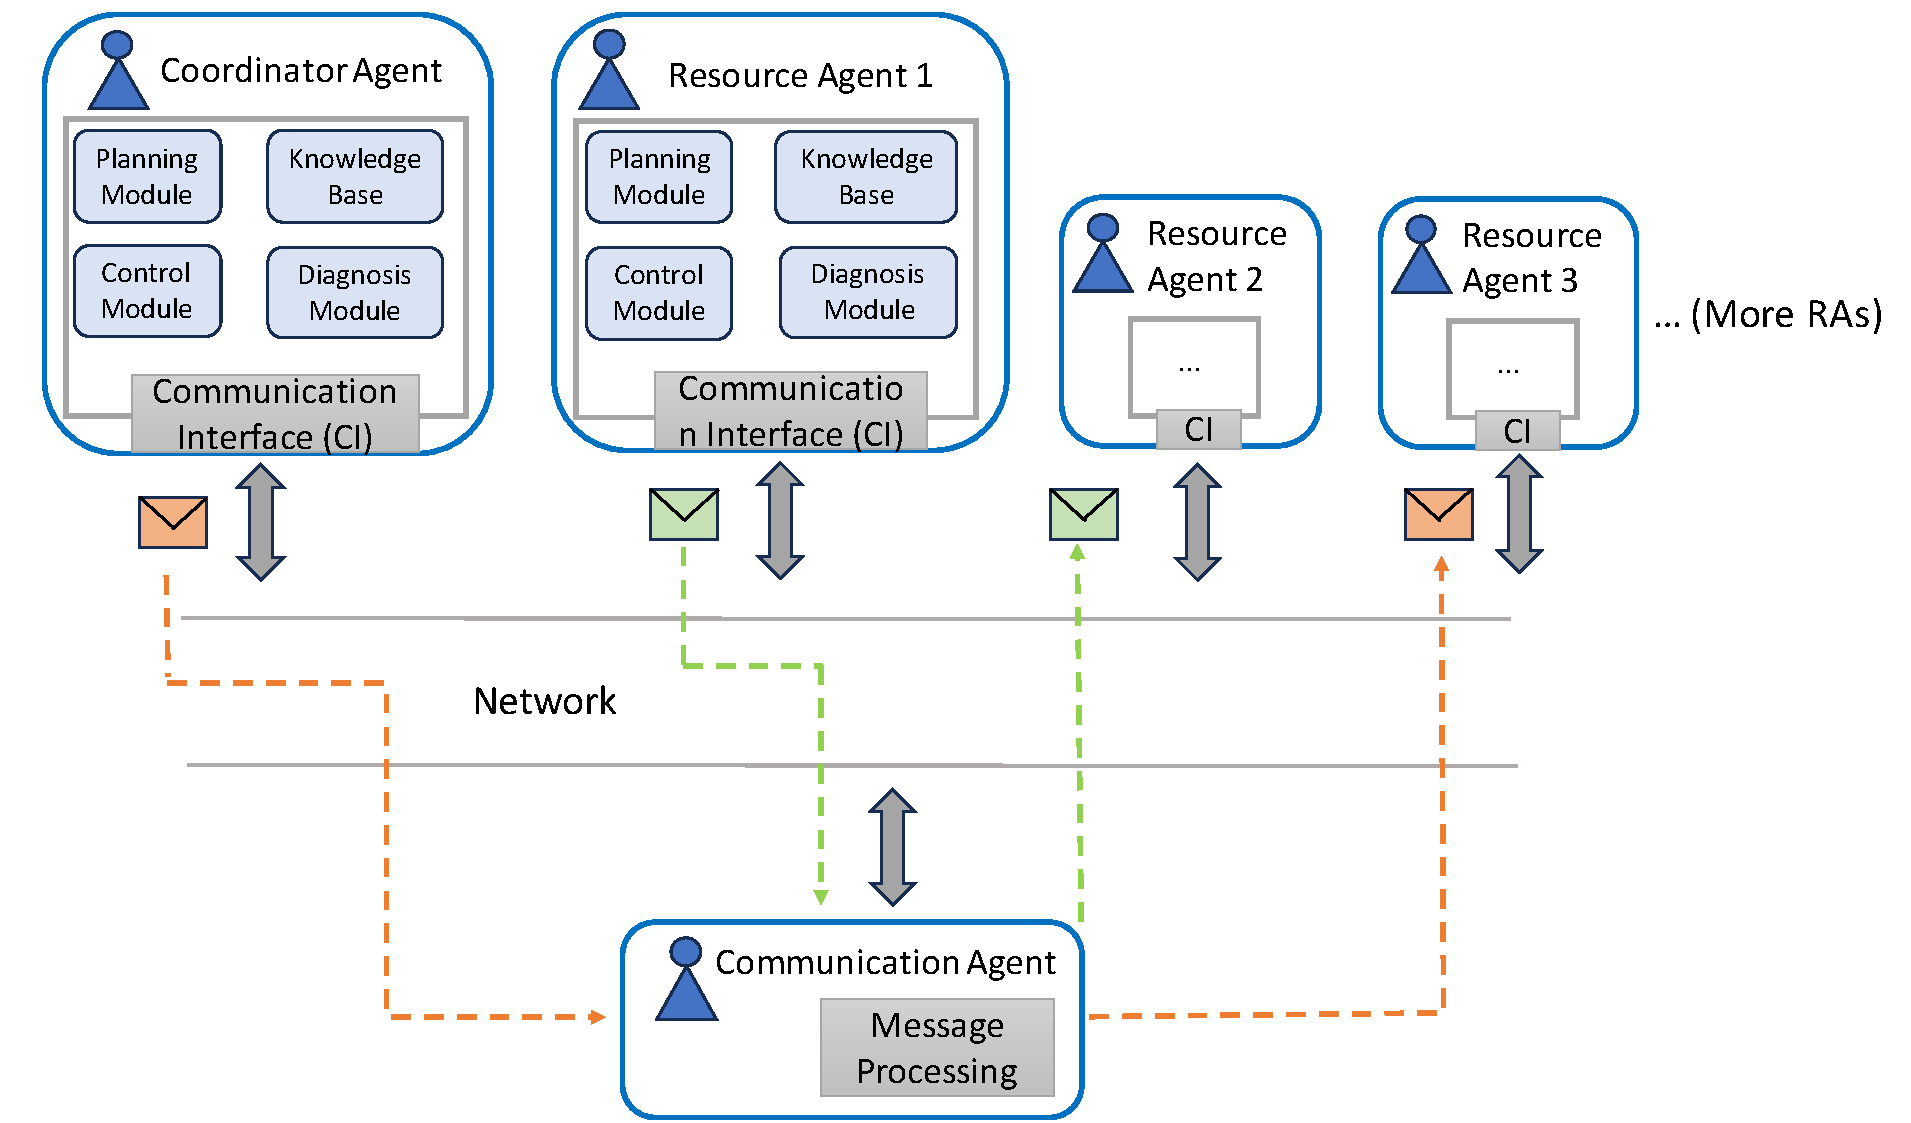
\includegraphics[width=\textwidth]{figures/MAS_Conceptual_Diagram.pdf}

\caption{Conceptual diagram of MAS.\label{fig: MASConceptual}}
\end{figure}

% decribe the conceptual diagram
For the modularization purposes, Wannagat's architecture is chosen for the 
system design because of its concentration on field-level operation over other 
design architectures, such as Fischer's and Ryashentseva's architecture that focus 
on higher levels in a production system.  
Fig.\ref{fig: MASConceptual} shows a conceptual diagram of a \gls{mas} based 
on the \gls{ra} design patterns 
in Wannagat's architecture\cite{cruz_salazar_cyber-physical_2019}, 
focusing on communication between agents, 
planning, and decision-making inside each agent. The \gls{cda} here is identical 
to \gls{ams} of Wannagat's architecture, which should also be considered an agent 
instead of a management system. The five modules within an agent are:

\begin{itemize}
    \item Planning Module
    \item Control Module
    \item Knowledge Base
    \item Diagnosis Module
    \item Communication Interface
\end{itemize}

for both \gls{cda} and \gls{ra}.
Based on these five modules, the agent tasks can be categorized into five parts. Some 
of them have been included in our \gls{mas}, while the others should be considered in the 
next design steps. 


Firstly, the planning module normally contains requirements like task planning, 
decision-making, 
resource allocation, sequencing, and scheduling. It has been mostly explored in our 
design, except for the communication Interface module. Inside a \gls{cda}, 
for task planning, we introduced 
a mechanism to break down tasks into smaller executable units (primitives). 
The decision 
making process is also enabled by including functionalities that can decide which task should be 
assigned to which agent based on the local \gls{db}. After that, for better resource 
allocation, the allocated agents will be assigned these tasks. What has not been 
considered is the scheduling tasks. It would be ideal if each agent could calculate 
the primitive execution time before starting.

Secondly, the control module should be able to perform tasks like monitoring, adaptation, 
control and optimization, resource allocation and actuation, and many more. The only part 
performed in our design is the actuation. All \gls{ras} can actuate the robot's operation 
unit by calling the primitive actuation functions. Other tasks, such as monitoring the 
robot states, adapting the plans with current states (e.g., emergent stop), and controlling and 
optimizing the robot's motion, are not under consideration in the work. 


The knowledge base module is another important module in general. 
The module consists of a lot of components and tasks, including \gls{db}, knowledge representation and reasoning, learning and knowledge 
sharing tasks. For DB design, it can be either hierarchical, relational, non-relational 
or object-oriented. In our work, the \gls{db} design of \gls{cda} is based on a 
hierarchical task decomposition structure. They are used to represent and reason task-related 
knowledges. 
Other parts, for example, learning from new tasks or sharing knowledge between agents, are not considered here.  


Although less concerned in the work, the diagnosis module is also important for fault 
detection, diagnosis and prediction, and root cause analysis and classification. Among all, 
only fault detection here is relevant to our work. In a \gls{ra}, an exception can be raised 
if the agents are currently not available or capable of primitives. 


The last module is the most important module in our case, which is responsible for agent 
communications. This module is embedded in each agent or as the main module in \gls{ca}. 
Common tasks, for example, are message parsing and encoding, connection 
establishment, message handling, message queuing, and data security. 
All tasks are executed at least once 
except for the security issues in our case. Here are some examples for each: 
messages are generally encoded and decoded into agent-specific data types, a stable 
connection can be ensured for constant data exchange, and messages can be prioritized in a 
queue inside a \gls{ca}. 


\subsection{\gls{osi} model and comparison between communication-relevant protocol layers}
%figure conceptual MAS
\begin{figure}[htbp]
    \centering
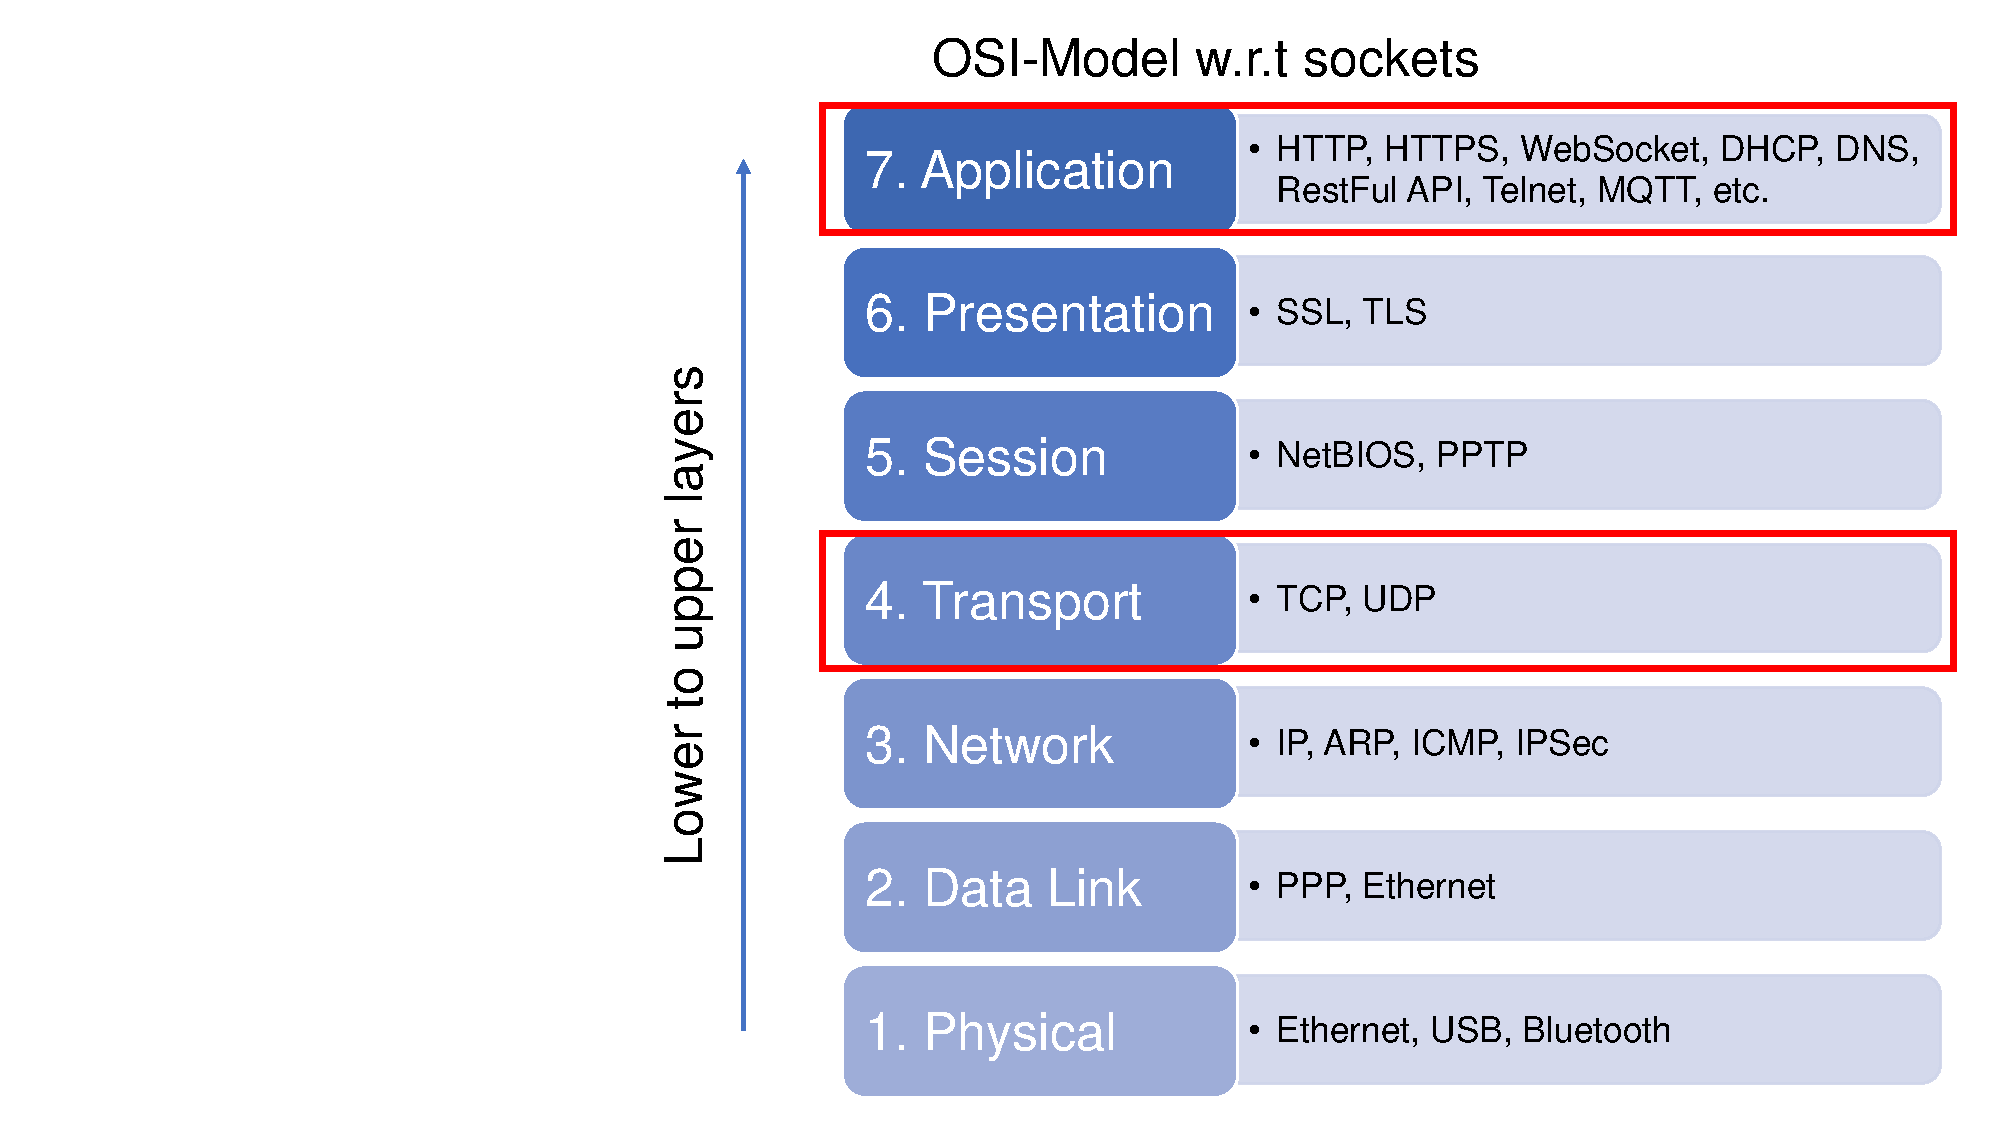
\includegraphics[width=0.6\textwidth]{figures/OSI.pdf}

\caption{\gls{osi} model with example protocols \label{fig: OSI}}
\end{figure}

An important aspect of agent communication is the communication protocols 
in different layers. 
Fig.\ref{fig: OSI} shows the famous \gls{osi} model with seven abstraction layers, with transport and 
application layers mostly relevant to network communication. TCP and UDP are typical transport layer 
protocols, and they provide a more abstract and generic service for reliable data transfer, 
while the application layer protocols like HTTP or Websocket are designed for applications with 
more user-specific functionalities. Although the application layer protocols are still based on 
TCP/UDP, they defined additional "rules" to 
specify the structure, content, and semantics of the messages transport. 


To choose one protocol over the others, we considered the Characteristics and compared 
those with our requirements of system design. Firstly, 
protocols within the same layer should be compared. In our studies, \gls{tcp} is chosen 
over \gls{udp}, while WebSocket is chosen over other comparable protocols 
such as \gls{http} and \gls{mqtt}. The decision is mainly made by comparison of their 
characteristics related to the design requirements. 



\subsubsection{TCP as transport layer communication protocols}
\gls{tcp} as a communication protocol is chosen based on the following characteristics: 
\begin{itemize}
    \item Use case
    \item Reliability
    \item Connection type
    \item Overhead 
    \item Sequence
    \item Retransmission of lost Packets
    \item Speed
    \item State
\end{itemize}
Normally, \gls{tcp} and \gls{udp} are used in different use cases with different focus. 
TCP is usually the communication protocol for email, text messages, and file transfers where a 
reliable connection is needed. It manages the pace of data transmission to avoid overload on 
the receiver side. Moreover, it stores information about the system to enable tracking. The 
packet loss rate is minimized in a reliable network configuration with the guarantee of the 
data retransmission mechanism and packet sequencing. However, it comes with the 
drawbacks. To ensure  
reliability, \gls{tcp} is designed with a larger overhead than \gls{udp}, which results in a 
lower data transmission speed. Besides, a three-handshake connection needs to be established, which adds up to extra delay. 


On the other hand, \gls{udp} is mostly used for live and real-time stream data transmission. 
Although suitable for real-time systems based on the stateless and connectionless 
properties and its lightweight overhead, \gls{udp} is not under consideration in our 
design based on its unreliability and non-sequencing properties. The packet loss rate is 
relatively higher because no retransmission of data is possible. Last but not the least, 
the packets may come in a different ordering, which results in problems in reconstructing 
data files at the receiver side.  

In a \gls{mas}, a reliable and direct communication between each agent should be 
guaranteed under a real-time requirement, 
which leads to the choice of \gls{tcp} over \gls{udp}. 
 


\subsubsection{WebSocket as application layer communication protocols}
Compared to transport layer protocols, application layer protocols provide more 
application-specific services. The choice of the protocols is again mainly based on the 
design requirements. Hence, three commonly used protocols, \gls{http}, 
WebSocket and \gls{mqtt} are compared horizontally with each other for their 
requirement-specific characteristics:

\begin{itemize}
    \item Use case
    \item Functionality
    \item Message patterns 
    \item Connection types
    \item State
    \item Overhead
    \item Real-time capability
    \item Flexibility
    \item Adaptability to dynamic changes
    \item Capability of handling instability
    \item Scalability
\end{itemize}

\gls{http}, a networking protocol, is widely used for web pages, images, videos, World 
Wide Web and many more. Its function operates in the following manners: a 
request-response-based message pattern that serves as the foundation for some third-party 
communication application such as RESTful API and used for the initial connection of WebSocket. The connection 
of \gls{http} protocol is non-persistent, and the connection will be closed after 
each individual request-response cycle. The communication is stateless, with additional 
overhead for each request-response cycle, especially for new connections. Therefore, 
it is less capable of handling real-time activities. Among all other protocols, 
\gls{http} benefits from its high flexibility in all environments, while in contrast, it is less 
adaptable to dynamic changes, less capable of stable connection, and less scalable 
in many cases compared to the other two protocols. 

Another option should be the WebSocket, which is, for example, used for chat 
applications and live gaming, providing a real-time, bi-directional, stateful, and full 
duplex communication 
solution. The term bi-directional means that, once the connection is established, 
either the client or the server can send a message to each other simultaneously, and the full-duplex indicates the independence of data flow in both directions. WebSocket is suitable 
for real-time applications because of its persistent connection, meaning that the connection 
will stay until it is closed. This mechanism greatly reduces the delay for 
reconnections. WebSocket also has the advantages of being highly flexible in most modern 
web browsers and many backend environments, its high adaptability, and scalability. The only 
drawback for the implementation of \gls{mas} could be its instability by constant disconnections. 


The last comparable protocol should be the \gls{mqtt} that is usually integrated into 
\gls{iot} with limited bandwidth. It has many leading points for 
\gls{mas} design. It is highly suitable for real-time systems with persistent connection, 
benefits from the statefulness property, and a minimal message overhead. The system 
based on \gls{mqtt} is highly real-time capable, flexible, adaptable to dynamic changes, 
capable of handling instability, and highly scalable on broker-client message transport. 
Nevertheless, it is not adapted for system design based on its publish-subscribe message pattern. 
As depicted in fig.\ref{fig: MsgConceptual}, the conceptual graph illustrates 
the differences between bi-directional 
full-duplex and other message patterns, such as Request-Response and Publish-Subscribe, 
in the context of data transport.
For the \gls{mqtt}, the publisher publishes (sends) a 
message within a topic to the broker (server), while the subscriber 
subscribes (receives) the message from the broker within the same topic. 
For response, a new topic needs to start, but there is no guarantee that the original publisher is listening, 
which is a drawback for send-and-receive patterns of \gls{mas}. 

Out of the three application layer protocols, we consider \gls{http} and 
WebSocket to be more appropriate for our 
\gls{mas} in the early design stage. The choice of using WebSocket will be verified 
by the test results with two protocols compared to each other in section \ref{chap: Result-RestFUL_WS}.


%figure conceptual application layer protocols
\begin{figure}[htb]
    \centering
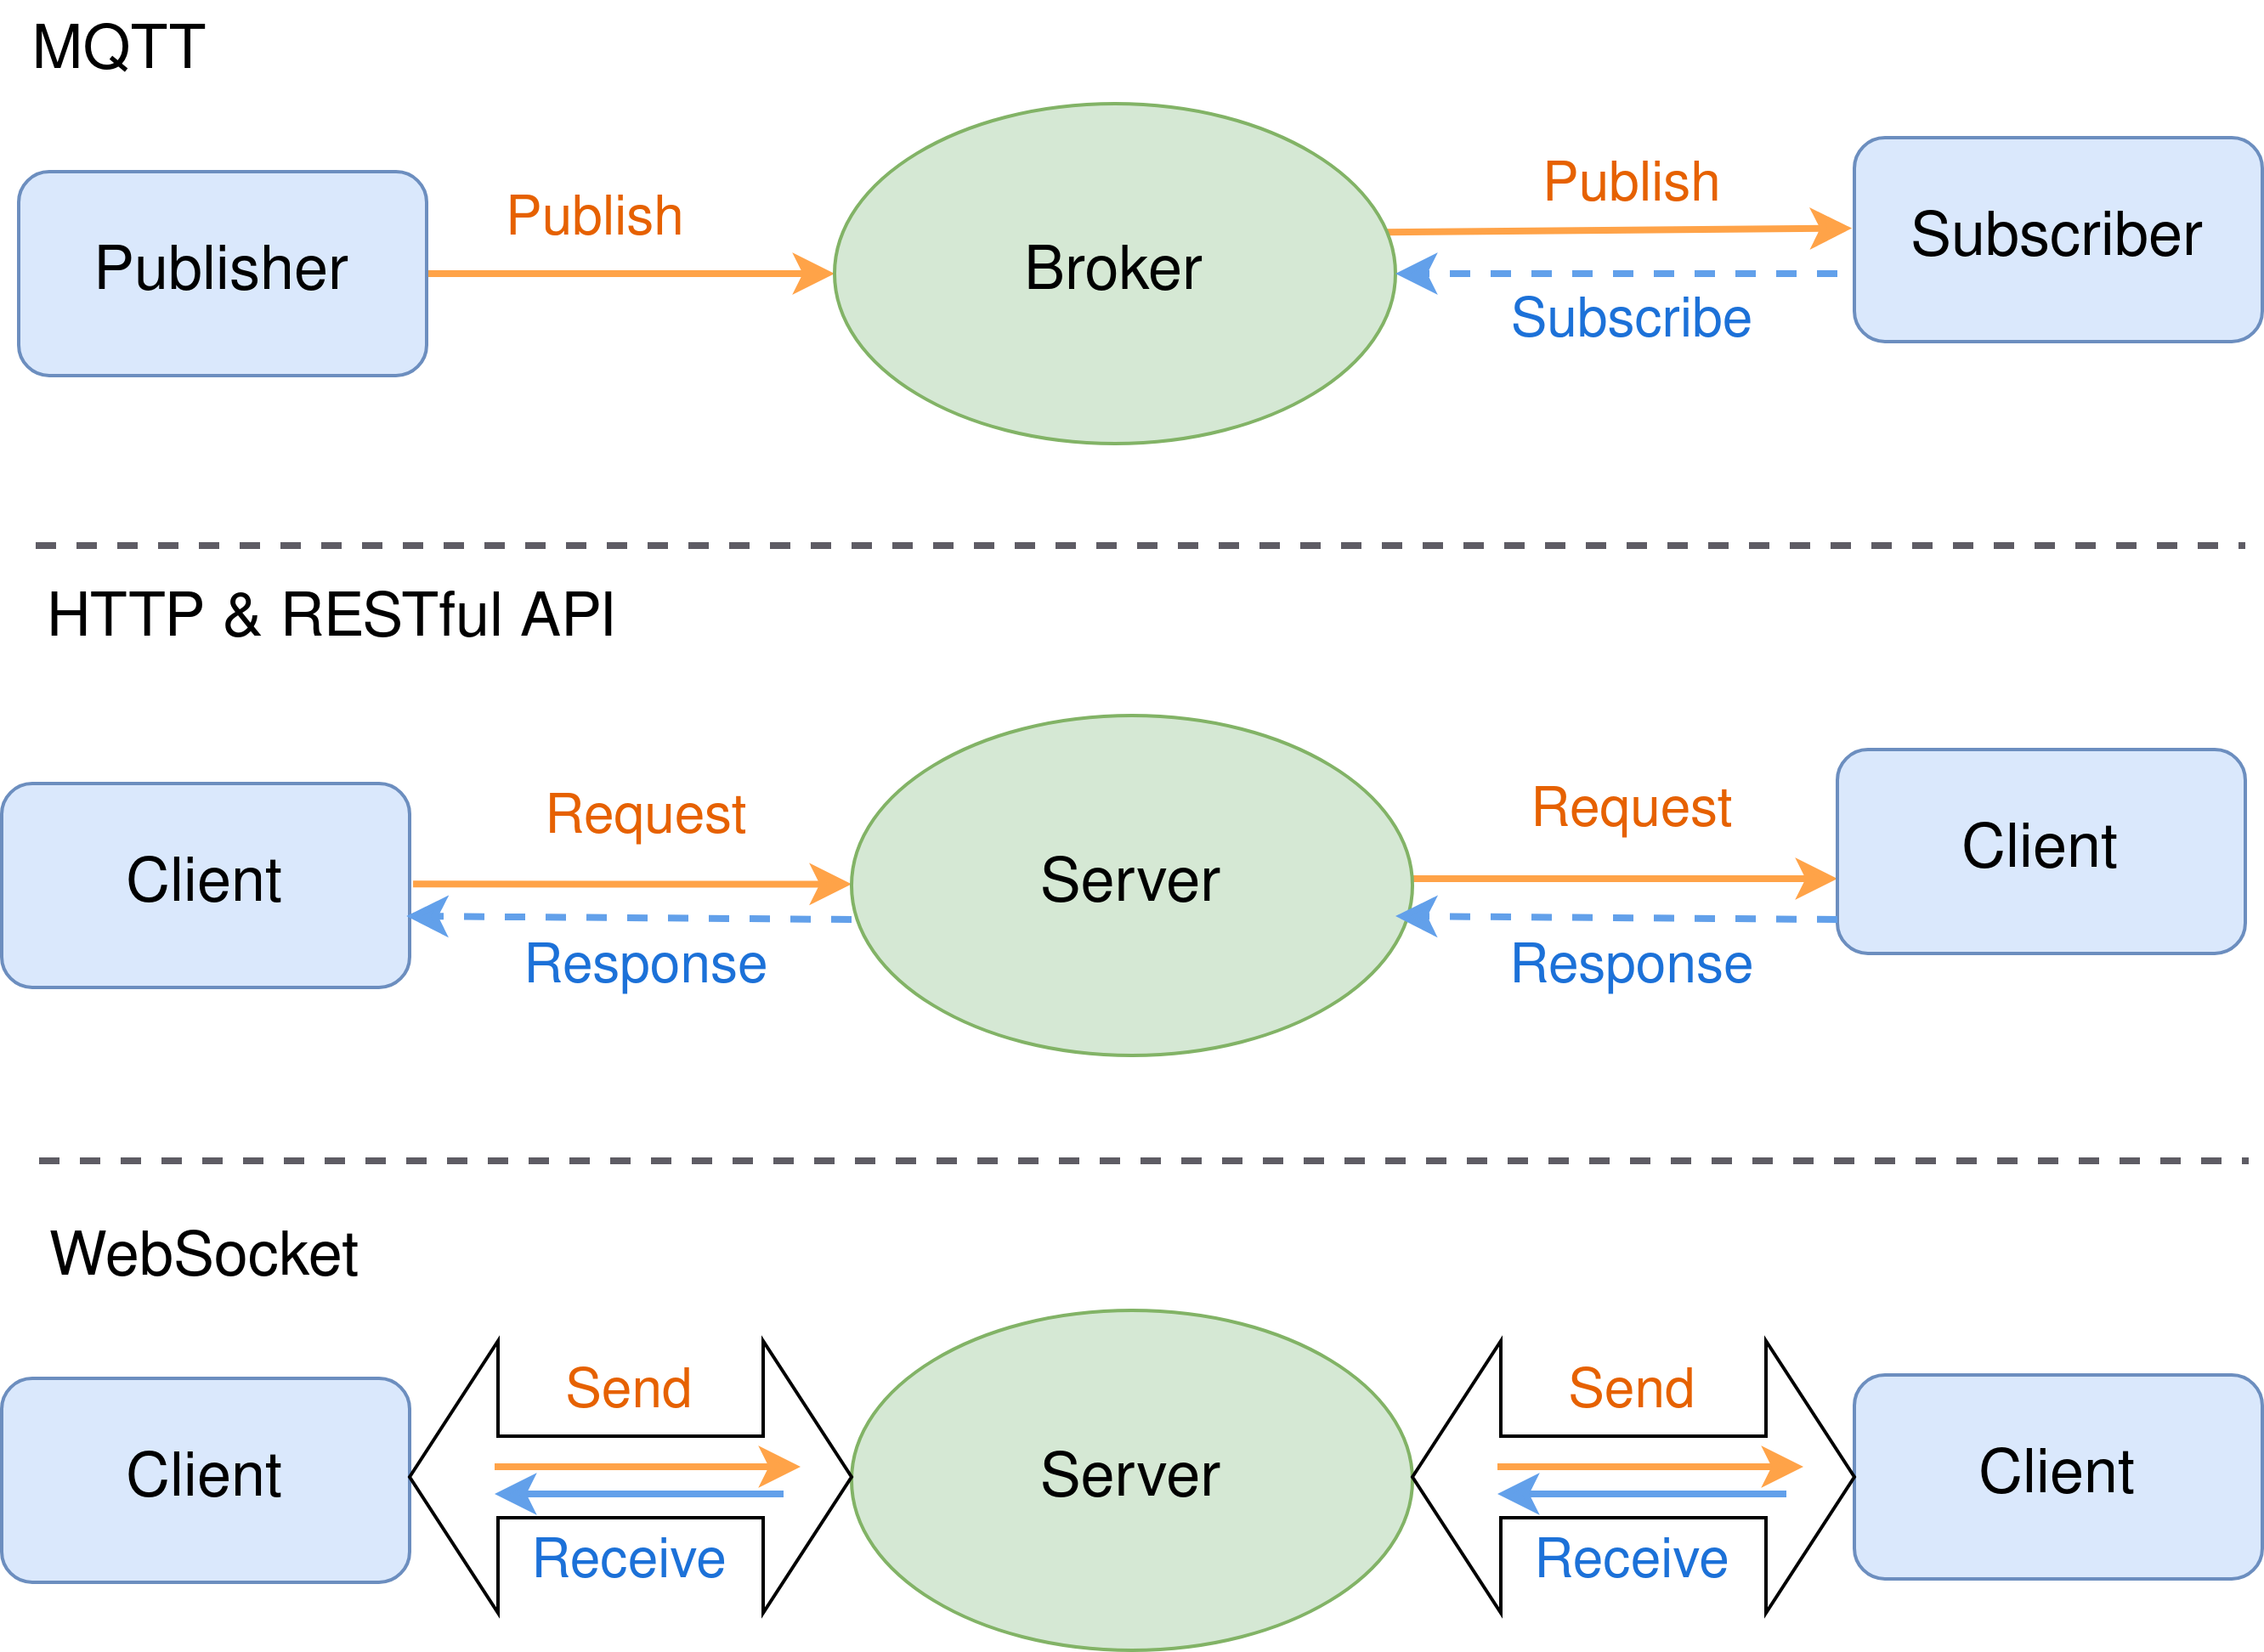
\includegraphics[width=0.8\textwidth]{figures/MessageConceptual.png}

\caption{Conceptual diagram of different application layer 
protocols\label{fig: MsgConceptual}}
\end{figure}





\subsection{Server-client design for \gls{mas} with the vertical comparison between WebSocket and \gls{tcp}}
In the final stage of the system design, WebSocket is chosen over \gls{tcp} as 
the base communication protocol for \gls{mas}. There are several reasons for this choice. 
A most basic communication mode according to \cite{vogel-heuser_delay_2023} 
is based on \gls{tcp} utilizing sockets (data transport endpoints in 
the program), which is beneficial for one-to-one 
or more-to-one, but never a more-to-more agent communication. This is based on 
the fact that client/-s should always start before the server. Assume that 
each agent is both a server and a client at the same time; the more-to-more 
agent communication will greatly enhance the complexity of the data exchange 
and also consume too much \gls{cpu} power. To be more specific, for a 
system of five agents, each agent has at least four threads for communication, 
which enables the agent to switch between the roles of clients and servers, 
making it impossible for real-time communication. The complex interconnections 
between agents are shown in fig.\ref{fig: threadMASConceptual}.

\begin{figure}[htb]
    \centering
    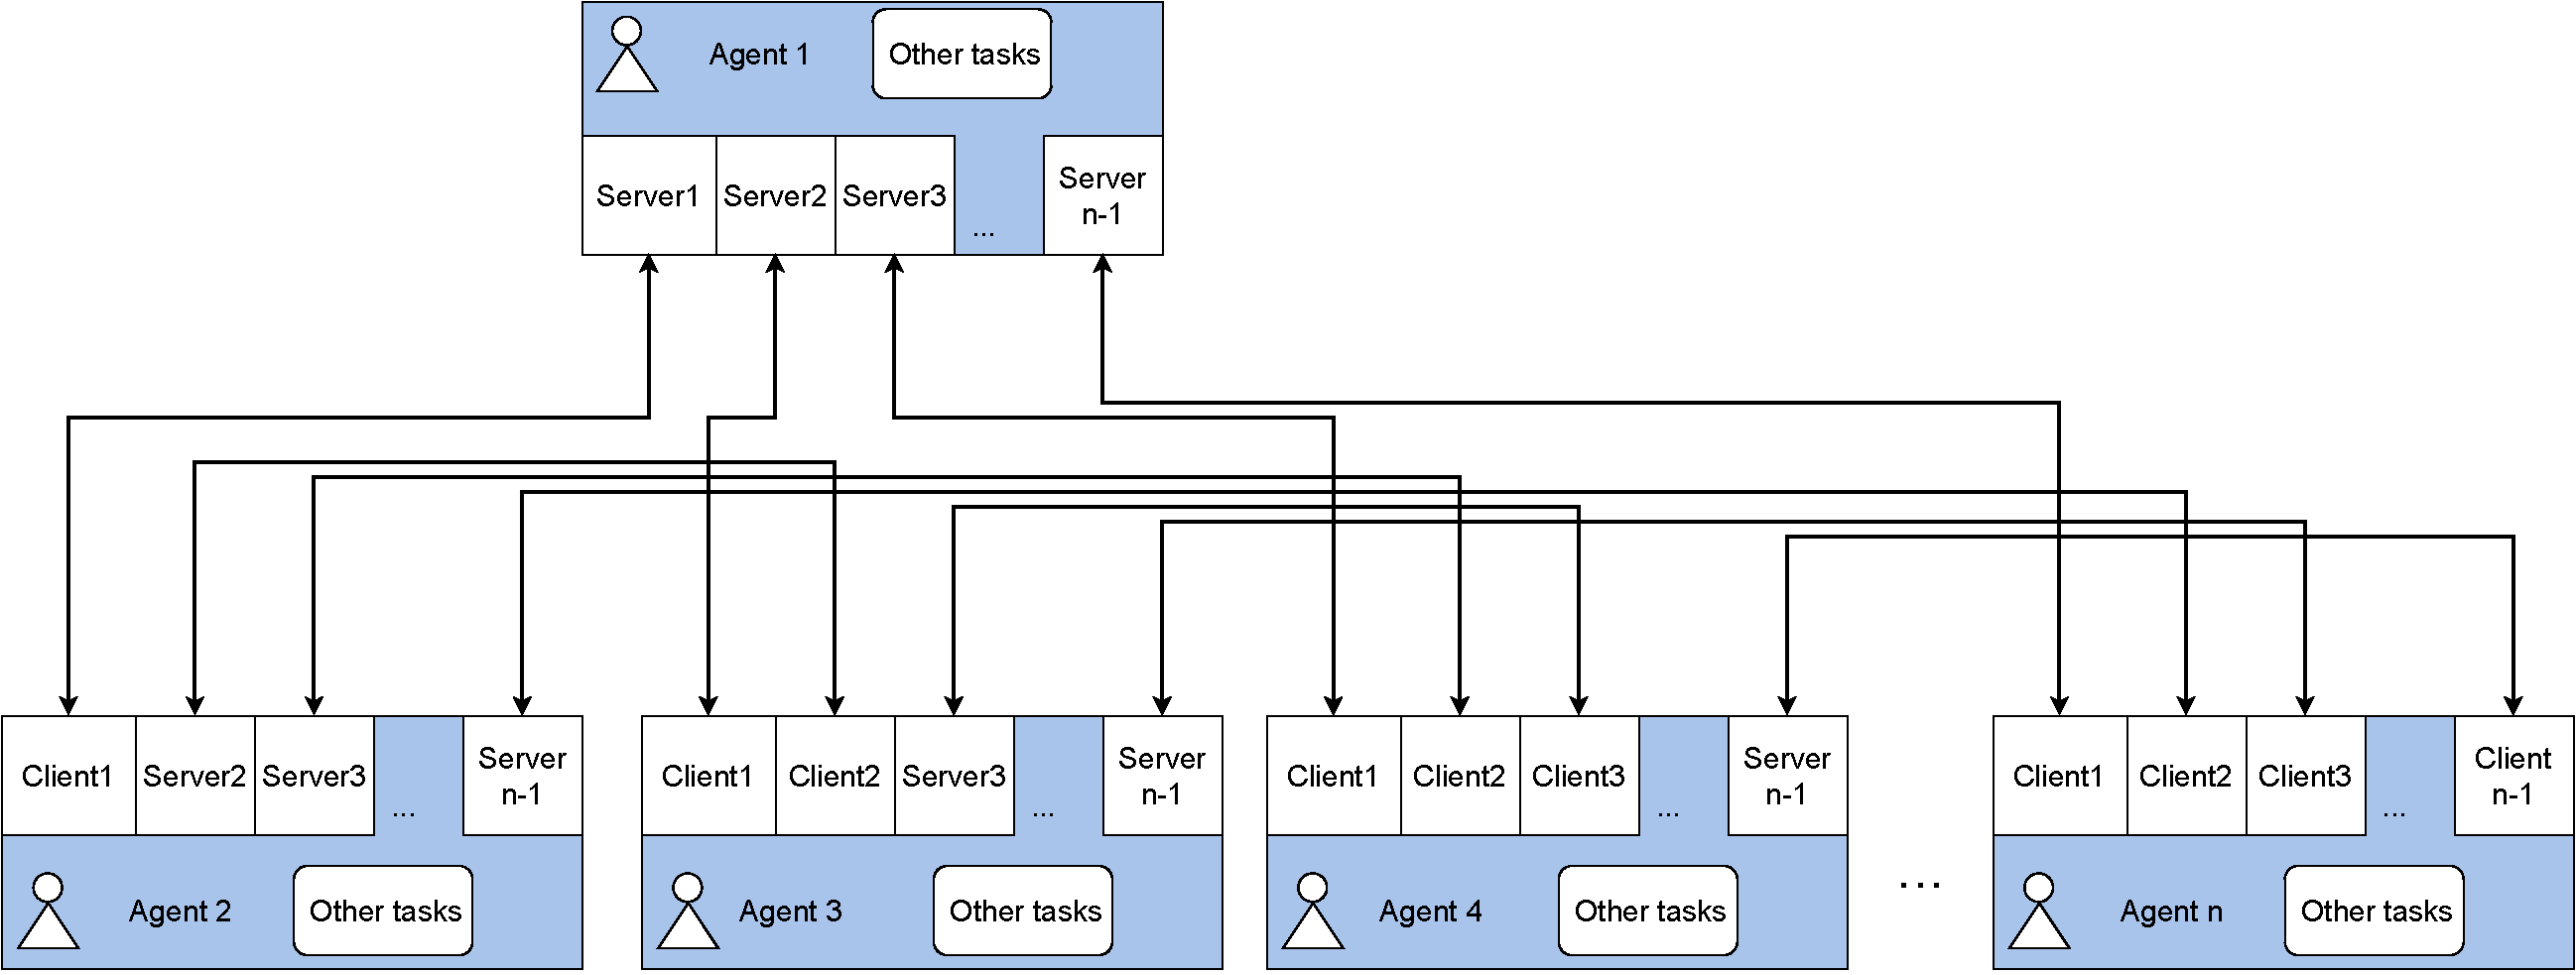
\includegraphics[width=\textwidth]{figures/threads_MAS.pdf}

    \caption{Conceptual diagram of \gls{mas} communication based on 
    \gls{tcp} sockets, an agent can be either a client or server by creating 
    multiple threads in a single script. \label{fig: threadMASConceptual}}
\end{figure}



After some unfeasible attempts, the demand to design a \gls{ca} to collect 
messages from sender agents, process them, and further transport them to the 
receiver agents has increased. Therefore, a server built with WebSocket serves 
as the \gls{ca}. Since the server should have many additional 
capabilities, including queuing messages, providing simple APIs for sending 
and receiving messages, and many more, raw bytes transport with \gls{tcp} is 
less under consideration for a complex \gls{mas}. However, \gls{tcp} socket 
may be more suitable for more-to-one communication for \gls{dta}, 
with its details described in section \ref{chap: RCPTCP-DTAPI}.  



\subsection{Scale out \gls{mas} communication with more than one server}
After choosing server-based \gls{ca} design and selecting WebSocket as the 
communication protocol for \gls{mas}, we now focus on system decentralization.  
Except for the ideas of the decentralization of tasks for each sub-agent, the agent 
communication system can also be decentralized. For example, represented as \gls{ca}, 
a server is responsible for handling all connections asynchronously, which should be 
feasible if the total number of agents does not exceed the limit. However, as already 
tested in our \gls{mas} design, a server cannot handle up to 1000 agents simultaneously. 
Hence, a distribution of a large communication system is necessary. 


However, it is challenging to distribute an agent communication system. 
Each agent needs to know 
with which server it should connect to and for what type of tasks. Another issue could 
be that if an agent receives conflicting messages from different servers, it will probably 
perform incorrect actions. A possible way is to design a mechanism to predefine the 
agent interaction to avoid system inconsistency. In our use cases, the communication 
between \gls{ca} and \gls{ras} and the interactions among \gls{ras} can be separated. 
The communication between \gls{ca} and other \gls{ras} is always under a central server, 
while the production-oriented communications between each \gls{ra} will go through a 
sublevel server. Although we have only two servers in our study, the number of servers 
can be expanded according to the scale of the \gls{mas}. For instance, if some agents 
never access other parts of agents during the production process, a subserver should 
be designed to connect those agents and keep the communications internal. Meanwhile, on 
the other hand, the integration of additional servers will increase the system complexity 
and introduce additional load balancing and synchronization issues. Therefore, 
in practical applications, engineers should be more careful in scaling the system in 
the design phase. Fig.\ref{fig: server-client-decentralization} shows the decentralization 
of the agent communication system with two servers. 

\begin{figure}[htbp]
    \centering
    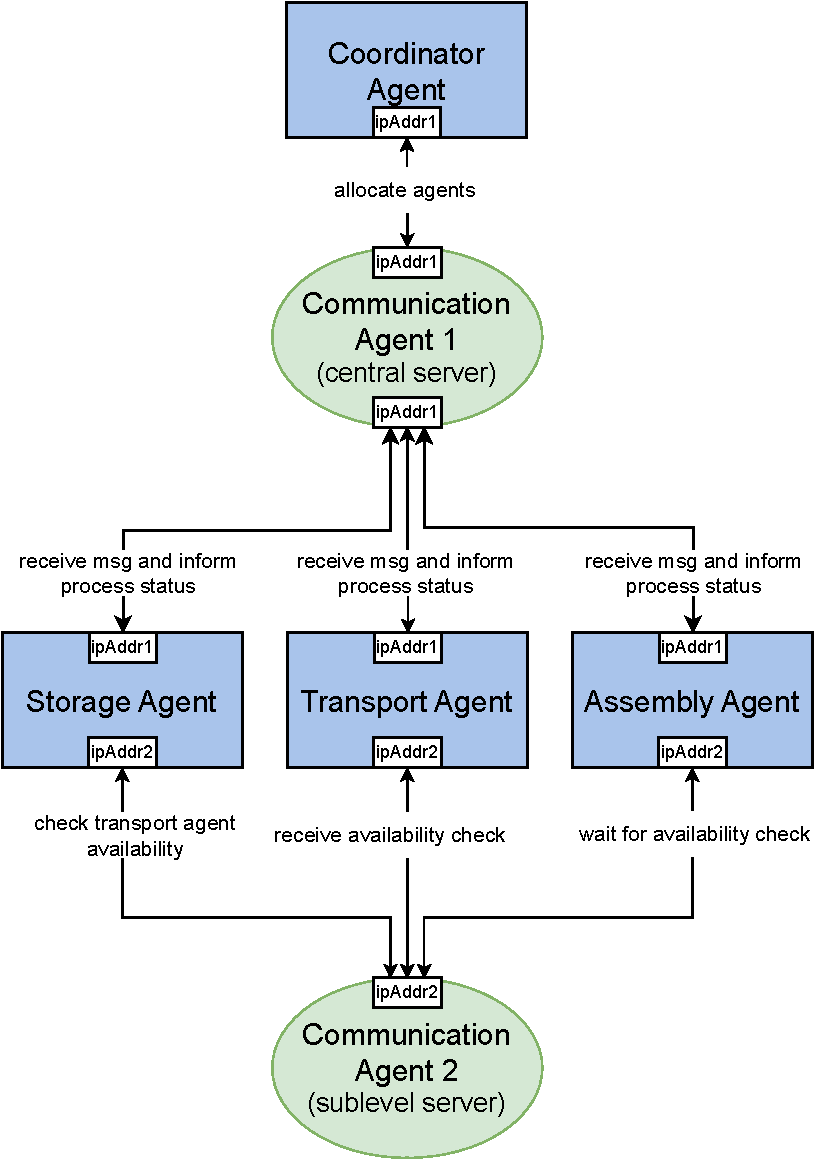
\includegraphics[width=0.7\textwidth]{figures/Server-clients-decentralize.pdf}

    \caption{Conceptual diagram of a decentralized \gls{mas} communication system with 
    two servers integrated.
    \label{fig: server-client-decentralization}}
\end{figure}





\subsection{Prerequisite}
\subsubsection{\gls{mas} system setup}
 

\begin{figure}[htbp]
    \centering
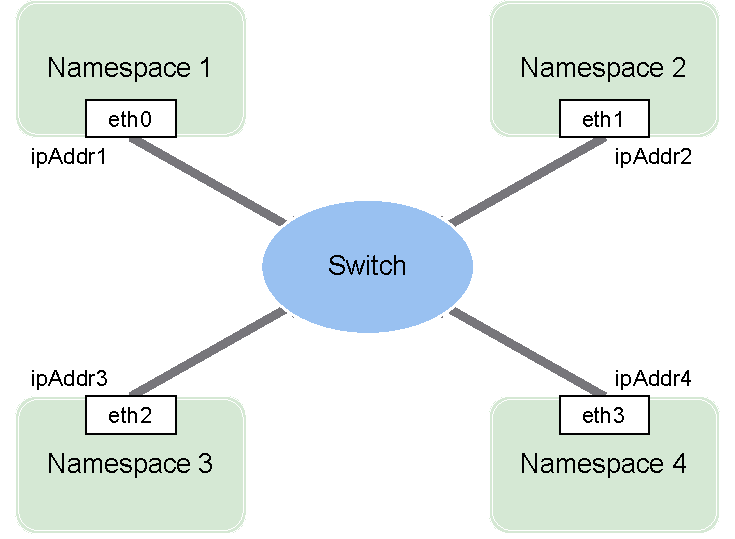
\includegraphics[width=0.8\textwidth]{figures/NamespaceConceptual.pdf}
\caption{Conceptual diagram of namespaces creation.
\label{fig: NSConceptual}}
\end{figure}

After choosing the suitable design architecture and protocols, the detailed 
software design for \gls{mas} and performance testing methods will be described below. 

Before simulating network environments for agent communication testing 
and development of the \gls{mas}, the internal packet routing between agents 
in a single Linux device should be avoided. A common way to visualize 
the network for performance testing is to use namespaces for network 
emulation. The trick is that a process running within a given
namespace will see only the network interfaces, including, for example, 
virtual interfaces and forwarding tables, that exist in that namespace. 
The applications under test should serve as a
switch, and each packet should be routed through these interfaces. 
Fig.\ref{fig: NSConceptual} shows that each namespace is assigned 
a virtual ethernet interface, 
starting with the name eth, along with an individual IP address. 
Each time a script gets called, it runs under a namespace with its 
IP address. In exercise, if a packet is sent from
Namespace 1 to 3 and then back; it is routed by the switch instead of 
bridges between namespaces to avoid internal routing. This external routing 
device is useful for delay measurement between each agent through the 5G network 
by introducing external delays to estimate the network environment. 

\subsection{Use WebSocket and RESTful API libraries for data transmission}
Since the programs are written in Python language, the python \textit{websockets} 
and \textit{flask} library can be used for WebSocket and RESTful API implementation 
respectively, resulting in different communication mechanisms. 


The connection establishment in WebSocket is rather simple. The program is 
built under the default \textit{asyncio} I/O framework, which 
provides a coroutine-based API for the server to handle multiple clients 
concurrently. The following steps 
show the simplified function calls for each connection step from the client side: 
\begin{enumerate}
    \item use \textit{with connect(URI) as websocket}: to establish connection with server
    \item use \textit{await websocket.send(client ID)} to send client ID to the server
    \item use \textit{await websocket.send(message)} to send messages to server
    \item use \textit{await websocket.recv(response)} to get response from server
\end{enumerate}
If the functions are called under a loop, the client can send and receive 
messages consistently until the connection is closed explicitly. 
Due to its statelessness, the client-relevant information (i.e., client ID) 
should be sent first. Since the server side is also running the same send 
and receive functions as in client; it will receive the message from the 
client, extract the receiver information, and route the packet continuously. 
So, at the receiver side, the send and receive calls are reverted: 
\begin{enumerate}
    \item use \textit{with connect(URI) as websocket}: to establish connection with server
    \item use \textit{await websocket.recv(response)} to receive messages from server
    \item use \textit{await websocket.send(message)} to send response to server
\end{enumerate}

With regards to the \textit{flask} APIs, it is closely related to the common 
\gls{http} request methods: GET, POST, PU, DELETE, PATCH, and HEAD. 
The client should POST and GET the message to and from the server, with 
a response indicating whether the function call is successful or not. The 
other client should then GET first and then POST a message back.  

\begin{enumerate}
    \item use \textit{$response = requests.post(f'{server\_address}/send\_message', json=data)$} to POST a message to server
    \item use \textit{$response = requests.get(f'{server\_address}/get\_messages/{self\_client\_name}$)} to GET a message from server
\end{enumerate}

At the server side, functions to process data and give responses are defined as:
\begin{enumerate}
    \item use \textit{$@app.route('/send\_message', methods=['POST'])$} to receive message from sender client
    \item use \textit{$@app.route('/get\_messages/<agent\_name>', methods=['GET'])$} to send message to receiver client
\end{enumerate}

Unlike the persistent connection in WebSocket, RESTful API needs to create 
a new connection for each new message, which seems to be less suitable for real-time 
requirements. 





\section{Global Digital Twin} \label{chap: Meth-External}
In section \ref{chap: Overview-External}, the data flow for the external 
\gls{dta} system will be presented. Following that, section \ref{chap: ntpsetup} 
will explain the \gls{ntp} setup used to measure delays between local devices and 
the cloud. And then, section \ref{chap: tcpsocket} briefly introduces the 
connection establishment workflow utilizing \gls{tcp} sockets. Finally, the 
last section will cover the setup of the Azure \gls{dt} platform for data ingestion.



\subsection{Overview (conceptual diagram)}\label{chap: Overview-External}

%figure conceptual DT
\begin{figure}[htb]
    \centering
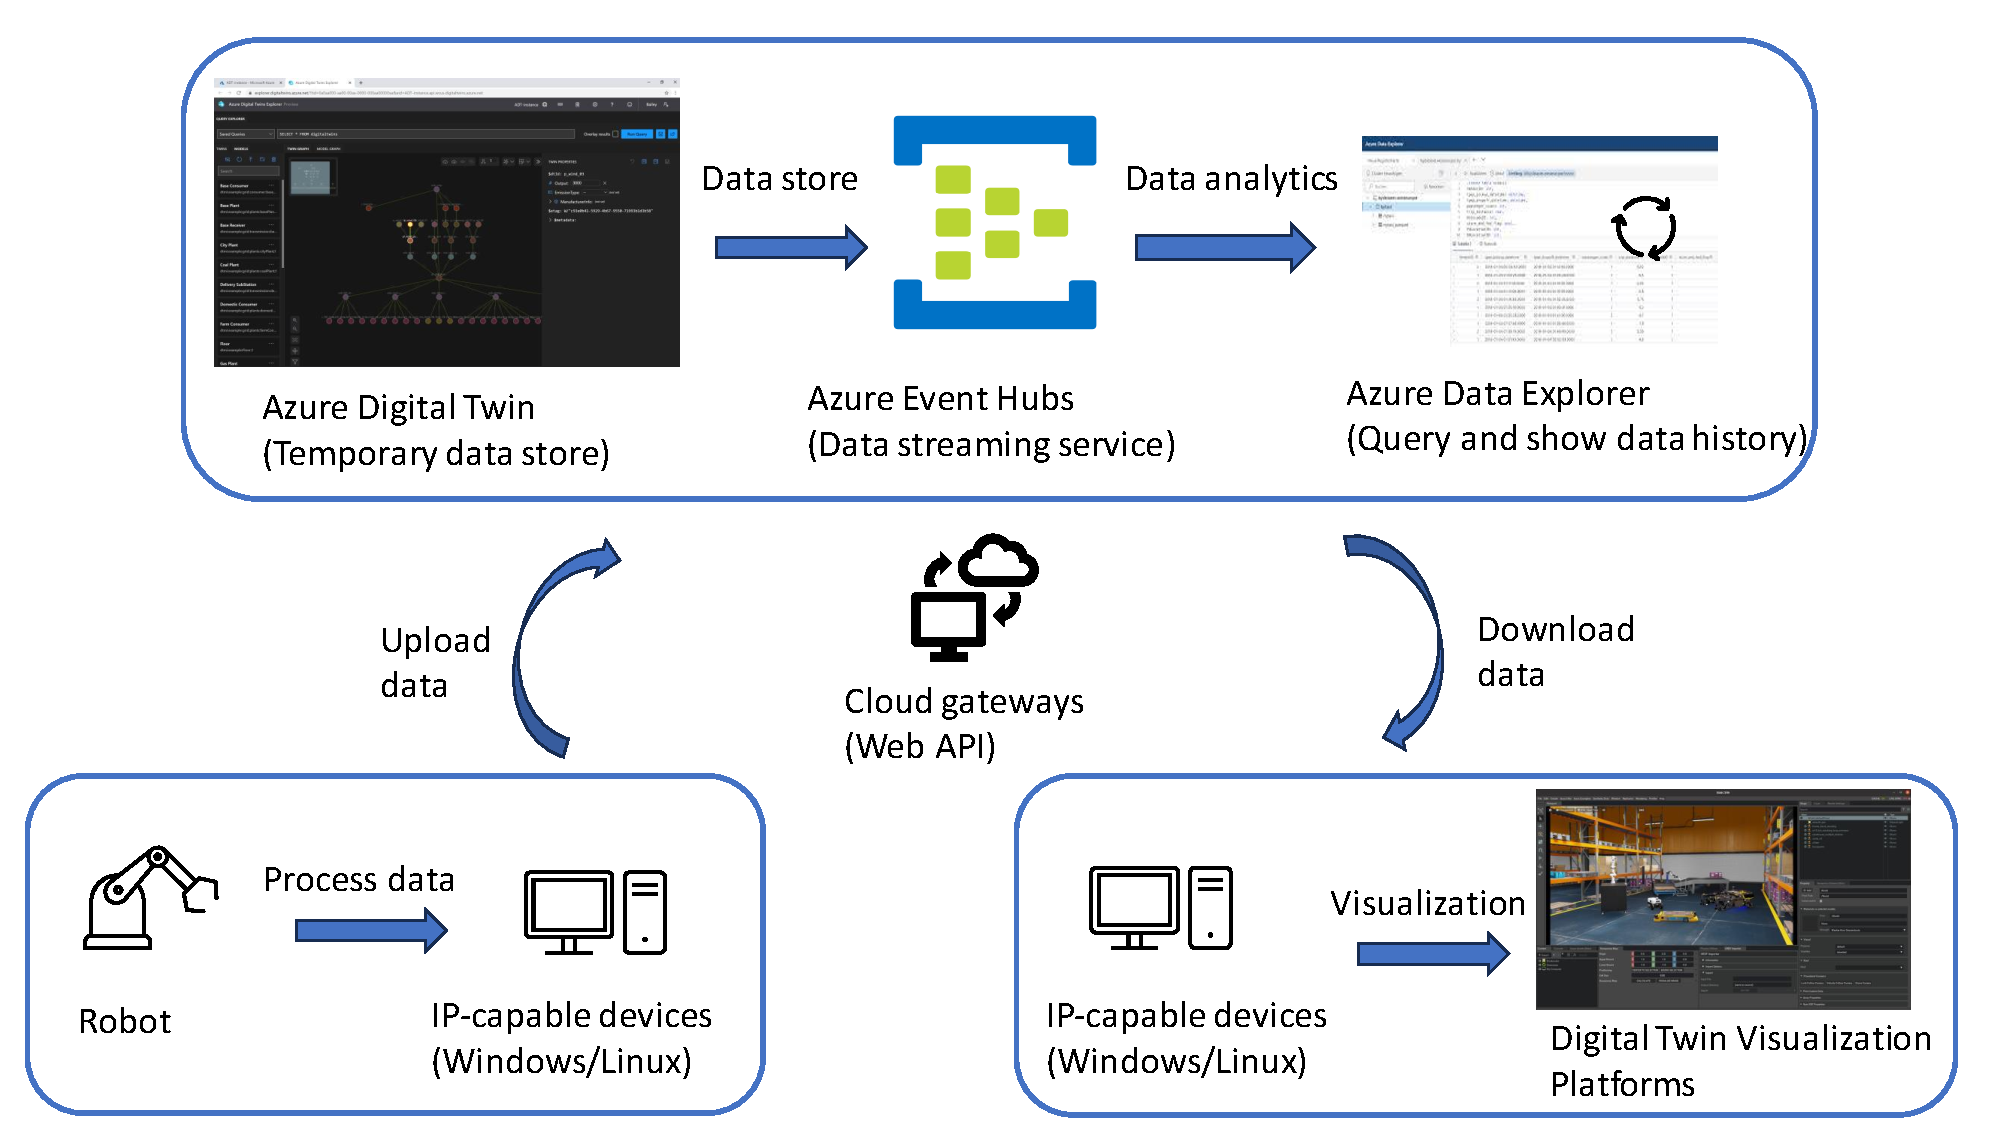
\includegraphics[width=\textwidth]{figures/DT_Conceptual_Diagram.pdf}
\caption{Conceptual diagram of global \gls{dt}. \label{fig: DTConceptual}}
\end{figure}

Named as DTAgent, \gls{dta} 
should also run on a Linux OS.
Despite being identified as an agent, \gls{dta} is not included in our 
\gls{mas} design. The main reason is that \gls{dta} receives process data from 
each robot right after the connection establishment with \gls{rcp} 
(program that controls the robot operation). Since the robot 
should always update its state, the \gls{dta} keeps alive even 
after the production finishes, making it possible to completely decouple 
both systems. If \gls{mas} breaks down, \gls{dta} can still tracks the robot 
states to find the potential issues. 


The workflow of updating global \gls{dt} through the \gls{dta} process is shown 
in Figure \ref{fig: DTConceptual}. The process begins on the left-hand side of the 
graph, where the \gls{dta} receives process data from robots, including steady-state 
data. The process data is parsed and uploaded one by one to the Azure \gls{dt} 
platform after separating the sticky packets from the \gls{tcp} socket.
All the updates of the \gls{dt} instances in the cloud are temporarily displayed 
in Azure \gls{dt} Explorer and concurrently stored in Azure Event Hubs. The history 
data can be ingested for further analysis in Azure Data Explorer. The Azure \gls{dt} 
Explorer serves as a robot status monitor, while Azure Data Explorer is a data analysis tool.
Once the remote data update is successful, the data is immediately downloaded to the local 
host and can be used as input for other visualization purposes. The real-time capability 
of this upload and download cycle of data should also be maintained.

It is important to note that the process data is generated by robot movement, 
which means that the \gls{dta} is completely independent of the \gls{mas}. This decoupling 
offers a 
significant advantage. Even if the \gls{mas} is in complete chaos, the robot's current status 
will still be captured and updated remotely. This is advantageous for both data acquisition 
and monitoring purposes.



\subsection{Prerequisite} \label{chap: ntpsetup}
\subsubsection{\gls{ntp} setup}
In order to measure the delays between the local host and cloud, the clock of both ends must be synchronized. 
Due to the nature of computer systems, the software clock might drift away from the "true" time (absolute \gls{utc}) 
due to various reasons like system load, hardware imperfections, or even temperature changes.
Therefore, before the measurement, the software clock of the local host should be synchronized with the global 
clock using \gls{ntp}. 
The \gls{ntp} setup of the Linux system is as follows:  

\begin{enumerate}
    \item System update and upgrade.
    \item Install \gls{ntp}.
    \item Add reliable global \gls{ntp} servers/server pools to configure ntp.conf file.
    \item Allow port 123/udp for or disable firewall.
    \item Restart \gls{ntp} and check \gls{ntp} status.
    \item Check synchronization status (e.g.: reach, delay, offset and jitter, etc).
    \end{enumerate}

Since the cloud system clock is already synchronized with \gls{utc}, all the tests and calculations results are based on \gls{utc}. 


\subsection{Connection establishment based on \gls{tcp} socket} \label{chap: tcpsocket}
Compared to WebSocket and RESTful API, the connection established with \gls{tcp} 
socket is relatively simple. Once the \gls{dta} runs as a server, it creates a \gls{tcp} socket 
object in a new thread, sends an arbitrary string to the \gls{rcp} client and 
waits for the initial "welcome" message from \gls{rcp} 
to confirm the successful connection. 
From the \gls{rcp} side, it also waits for the connection establishment before 
starting any robot control motions.  
In the \gls{dta}, there are multiple threads created to wait for the connection 
from \gls{ras}, such as the MiR600 transport agent and the storage agent. 
The \gls{dta} can run on the same device with \gls{rcp} or a device dedicated 
to receiving the robot's connections. The following fig.\ref{fig: tcpRCPDTA} shows the connection 
process of \gls{rcp} and \gls{dta}. 

\begin{figure}[htb]
    \centering
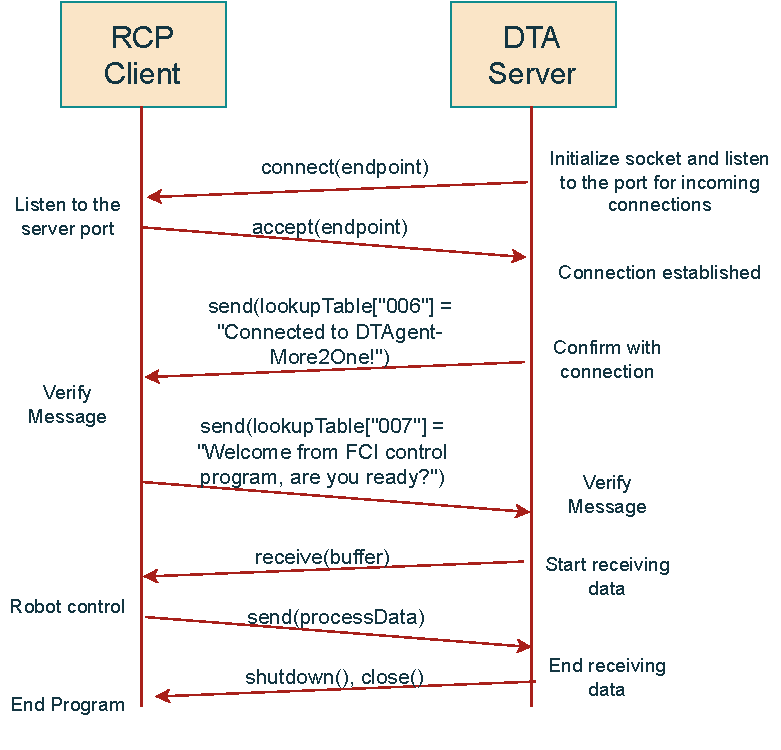
\includegraphics[width=0.8\textwidth]{figures/tcpsocket.pdf}
\caption{Connection process between \gls{rcp} and \gls{dta} 
through \gls{tcp} socket. \label{fig: tcpRCPDTA}}
\end{figure}


\subsection{Data flow with \gls{tcp} socket and Azure \gls{dt} REST APIs}\label{chap: RCPTCP-DTAPI}
Different from the \gls{mas} with frequent connection reestablishment and heavy data handling in \gls{ca}, 
\gls{dta} only conducts a simple one-way data flow, starting from \gls{rcp} and 
ending at local download from Azure \gls{dt} platform. \gls{tcp} is beneficial for 
it's less overhead and lightweight compared to WebSocket. 


The Azure \gls{dt} REST APIs are, on the other hand, responsible for the data 
transport between local devices and the cloud. It consists of two modules: the 
control plane APIs for managing \gls{dt} instances as a whole and the 
data plane APIs to manage elements of the Azure \gls{dt} instances. For the 
time measurement of \gls{dt} update, we mainly used the data plane APIs. The 
common operations include create, delete, update, and list. In the test, two 
APIs are mainly used. \textit{UpdateDigitalTwin} is used for updating 
the whole twin instance 
and \textit{UpdateComponent} for the specific update of \gls{dt} component. 
Other APIs, for example, \textit{Query}, are used to execute queries for twin 
instances to get the demanding components. It was once used for timestamp 
logging in local devices. 


\subsection{Azure \gls{dt}}
\subsubsection{Initial connection setup}
According to the workflow explained in section \ref{chap: Overview-External}, 
it is crucial to establish a reliable and operational Azure \gls{dt} platform 
to ensure seamless data transfer. The platform should include Azure \gls{dt} Explorer, 
Azure Event Hub, and Azure Data Explorer. Additionally, the Azure \gls{dt} 
instance must be configured with a time-series data history connection. Other resources 
must also be created, such as an Event Hubs namespace, an event hub, Azure Data Explorer 
cluster, and a database. To use the data update APIs 
from section \ref{chap: RCPTCP-DTAPI}, a client for Azure \gls{dt} should be 
initialized. The following steps should enable the Azure \gls{dt} connection 
establishment: 


\begin{enumerate}
    \item Initialize the URL that points to the Azure \gls{dt}
    \item Get a credential to authenticate with Azure services
    \item Create a client object that allows interaction between \gls{dta} and Azure \gls{dt}
    \end{enumerate}

After the connection from the local device to the Azure \gls{dt}, 
data is sent to an event hub, which eventually forwards the data to 
the Azure Data Explorer cluster and stores it in a database. The history data includes 
twin property updates, twin lifecycle events, and relationship lifecycle events, which 
can be later queried in Azure Data Explorer.


\subsubsection{Data history setup}
Here is the sequence of the basic setup in the Azure platform:
\begin{enumerate}
    \item Create Azure Event Hub namespace and add an instance.
    \item Create Azure Data Explorer cluster and add database.
    \item Connect data history of the Event Hub instance to the \gls{dt} instance.
\end{enumerate}

In order to verify whether the connection is successful, one can try updating the 
\gls{dt} instance and querying data from the Azure Data Explorer side. The query
language is called \gls{kql}, which is powerful for pattern discovery, anomalies 
and outliers identification, and statistical modeling (various graphs creation). 
Following algorithm \ref{alg: KQLCode} is a snippet of the example \gls{kql} code in the test: 

\begin{algorithm}
    \caption{\gls{kql} for Azure \gls{dt} data history query}
    \label{alg: KQLCode}
    \begin{algorithmic}
        \State  AdtPropertyEvents 
        \State {| where ID == 'RadPositionJoint3' and Key == 'value'}
        \State {| where TimeStamp between (datetime(2023-08-27 16:02) .. datetime(2023-08-27 19:00))}
        \State {| order by TimeStamp asc}
        \State {| project TimeStamp, Id, Key, Value}
    \end{algorithmic}
\end{algorithm}


\begin{figure}[htb]
    \centering
    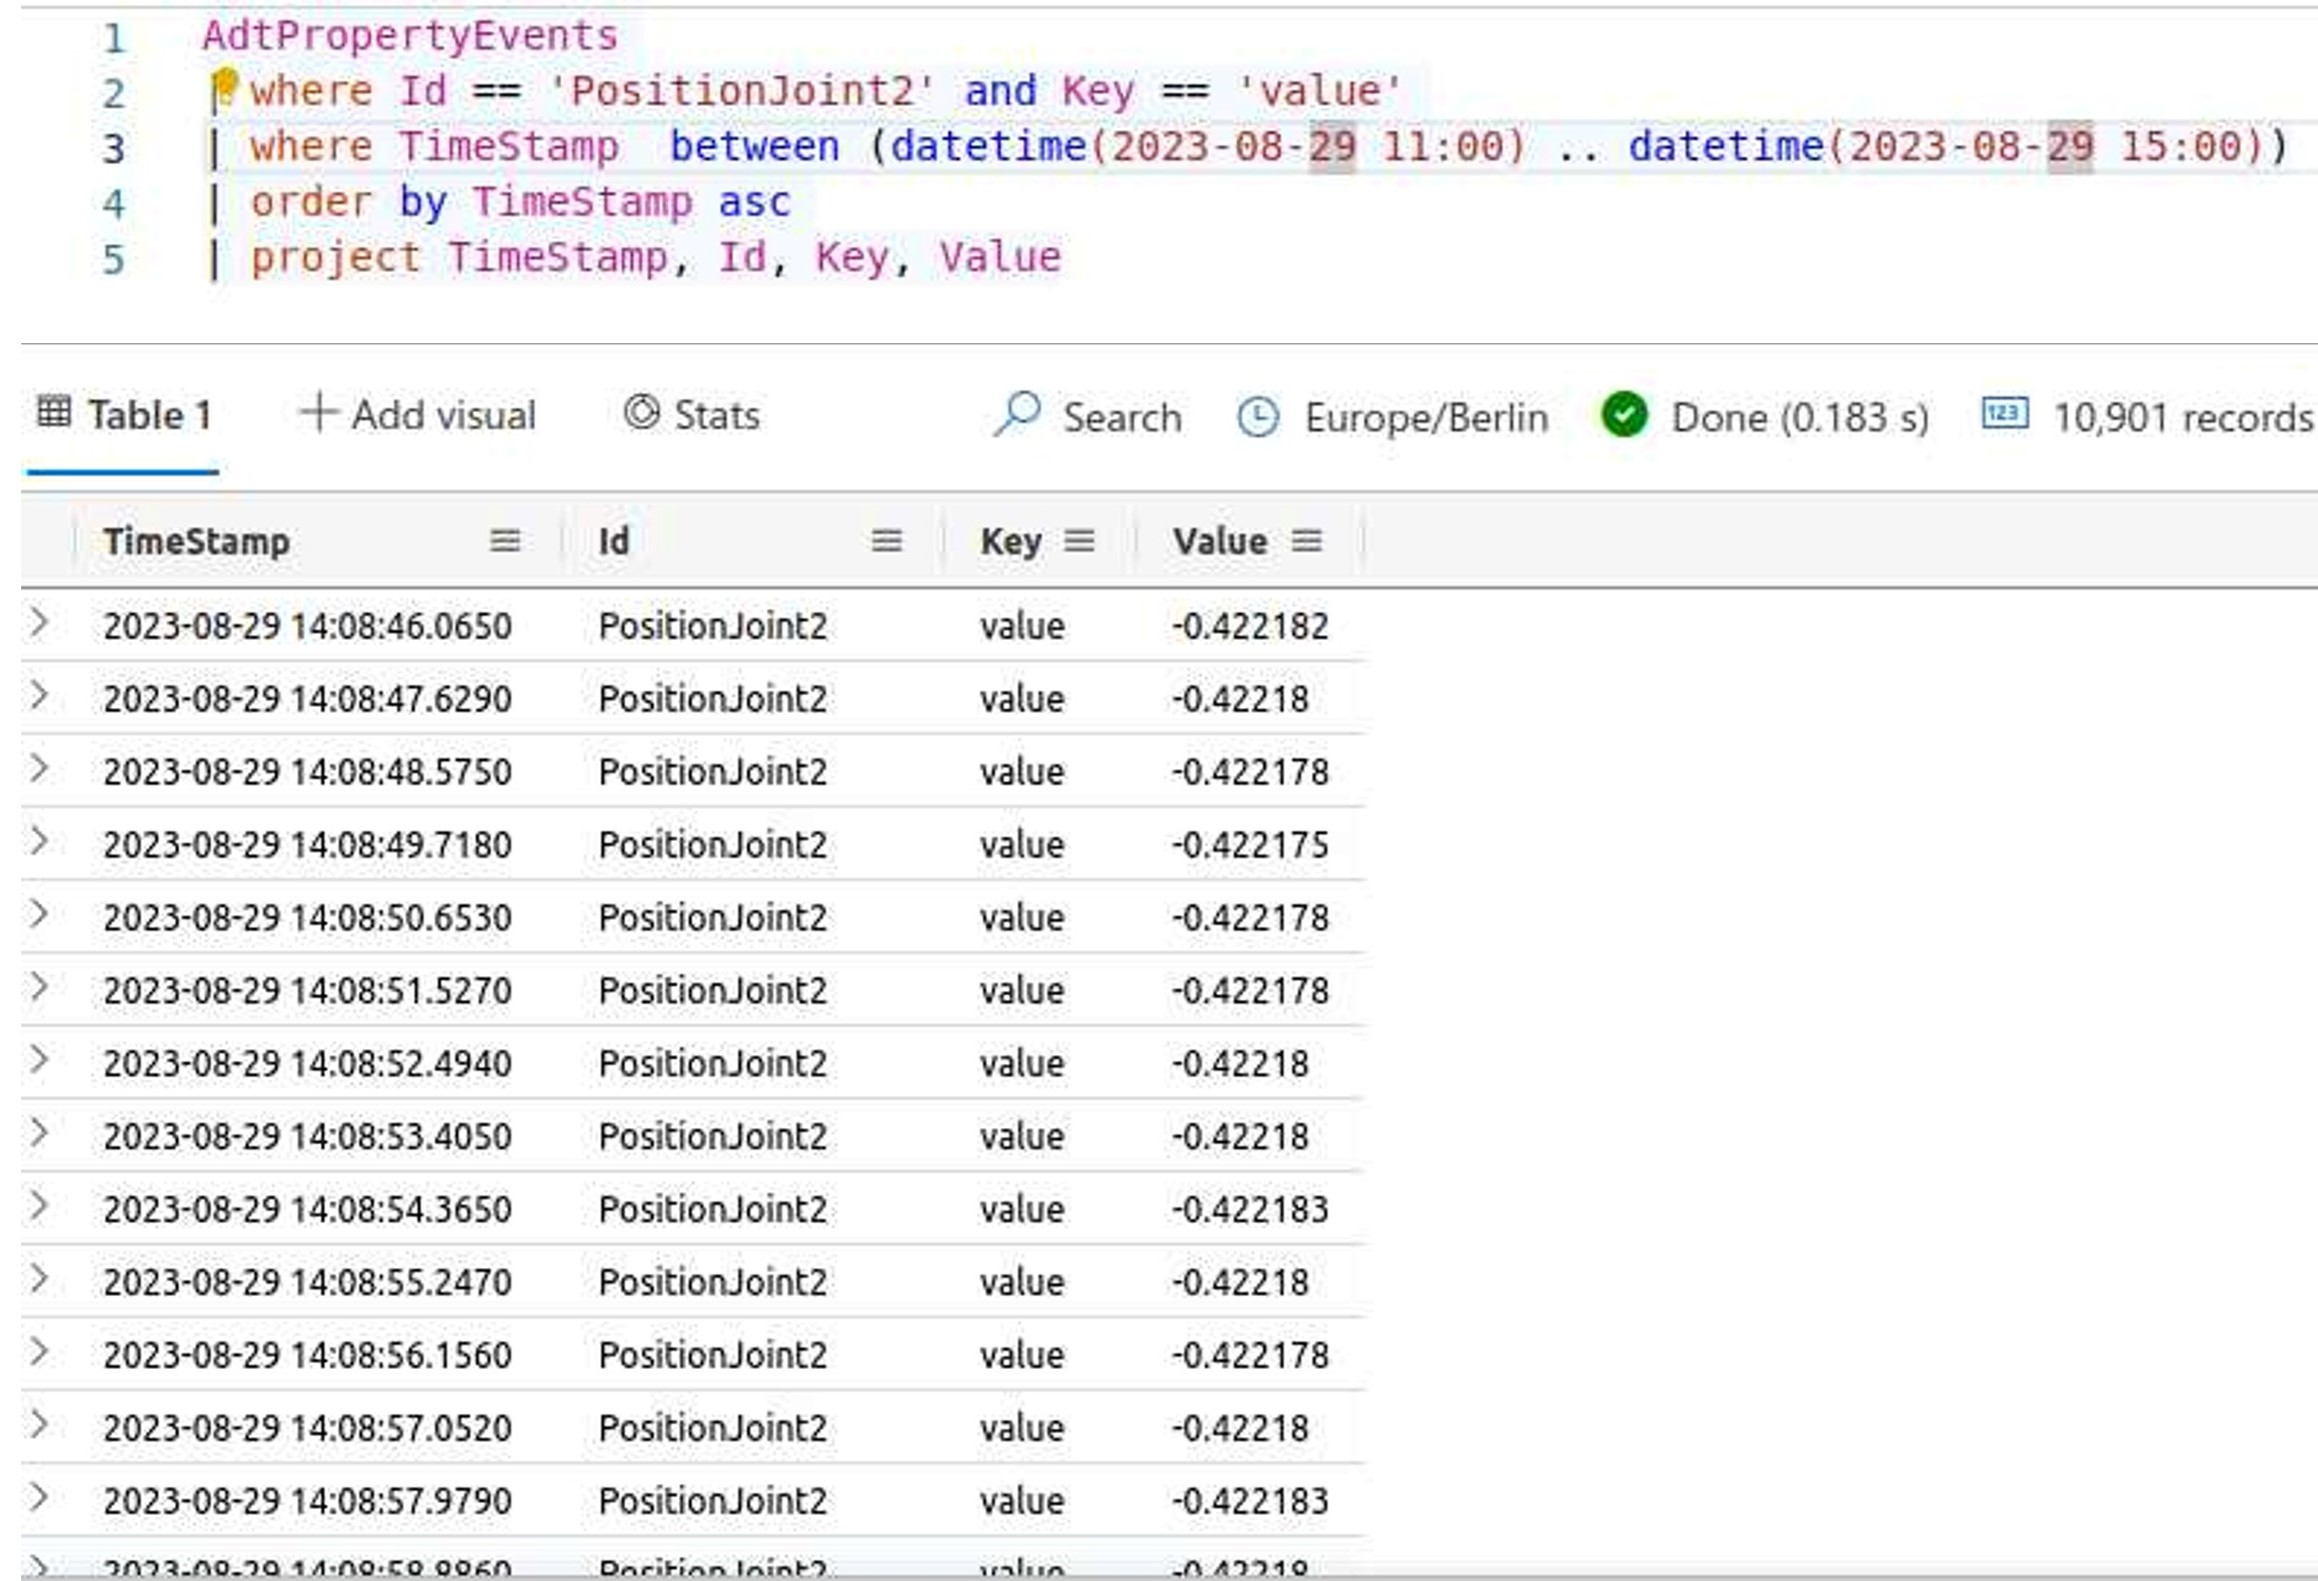
\includegraphics[width=0.8\textwidth]{figures/KQL_cut.jpg}
    \caption{An example of Azure Data Explorer with \gls{kql} to 
    query history data.\label{fig: KQL}}
\end{figure}

As shown in fig.\ref{fig: KQL}, by executing the code from the snippet, all the history data will be listed as a table 
which can be downloaded to the local devices later. 

\subsubsection{Large patch size for Azure \gls{dt} update}
One of our tests for differentiating the \gls{owd} for Azure 
\gls{dt} depends on patch size of the to-be-updated 
twin properties (section \ref{chap: Result-DTA-DT}). In the test, 
the small patch only contains the twin value, while the large patch 
contains more information under the architecture of the twin graph. 
The patch size can be extended by \textit{AppendAdd} to add more properties. 
In our test, for example, the twin's category, checksum, value type, 
value type, data specification, id and the semantic id value are added 
to greatly enlarge the patch.   

Fig.\ref{fig: largepatchDT} shows the update of the large patch of a 
twin in Azure \gls{dt} Explorer at the right hand side. 


\begin{figure}[htb]
    \centering
    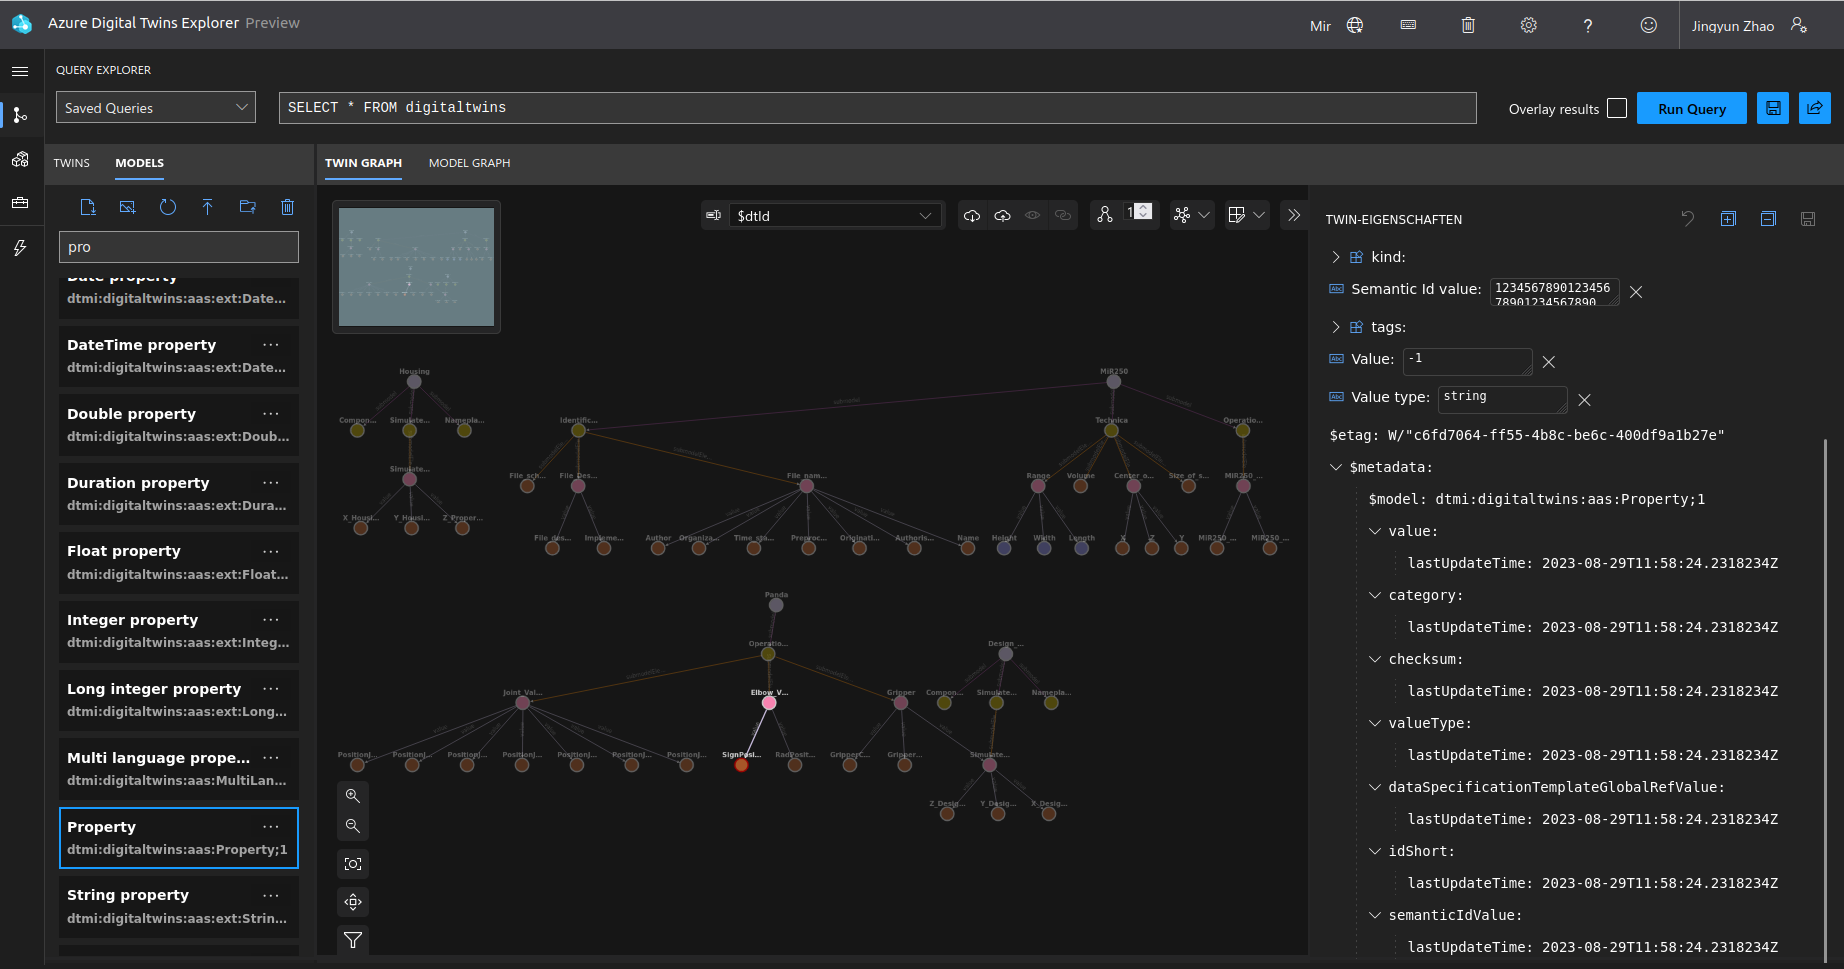
\includegraphics[width=\textwidth]{figures/Update_twin_largerPatch.png}
    \caption{An example of twin update in Azure \gls{dt} 
    Explorer with large patch.\label{fig: largepatchDT}}
\end{figure}




\section{Modularization}\label{chap: Meth-Modular}
In addition to the local \gls{mas} and global \gls{dt} designs of a general \gls{mas}, 
there are also some considerations of modularizing timing behaviors of the 
system. In the following sections, the \gls{tcp/ip} model as well as 
\gls{dsl} will be introduced and used as the design basis of a modularized general 
\gls{mas}. 
\subsection{From \gls{osi} model to \gls{tcp/ip} model}

Although TCP is classified as a transport layer protocol according to the 
\gls{osi} model (fig.\ref{fig: OSI}), data transport between different TCP sockets 
still involves all layers. This is because a program using socket libraries 
operates the TCP socket, which is an operation under the application layer. 
The transport layer protocols only accept data from the session layer in the 
\gls{osi} model and break it down into smaller pieces to ensure reliable and correct 
data transport. However, considering delays in all seven layers for modularization 
purposes would be too strict and complicated. Therefore, the focus should be 
shifted from the general \gls{osi} model to the more abstract TCP/IP model, as depicted 
in fig.\ref{fig: TCP_IP}.

The TCP/IP model consists of four layers: application layer, transport layer, 
internet layer, and network access layer, with each mapping different layers in 
the \gls{osi} model. As depicted in the TCP/IP model, the application layer roughly 
contains the upper three layers, while the network access layer contains the 
physical and data link layers. The network layer is renamed as the internet 
layer, while the transport layer remains the same.

\begin{figure}[htb]
    \centering
    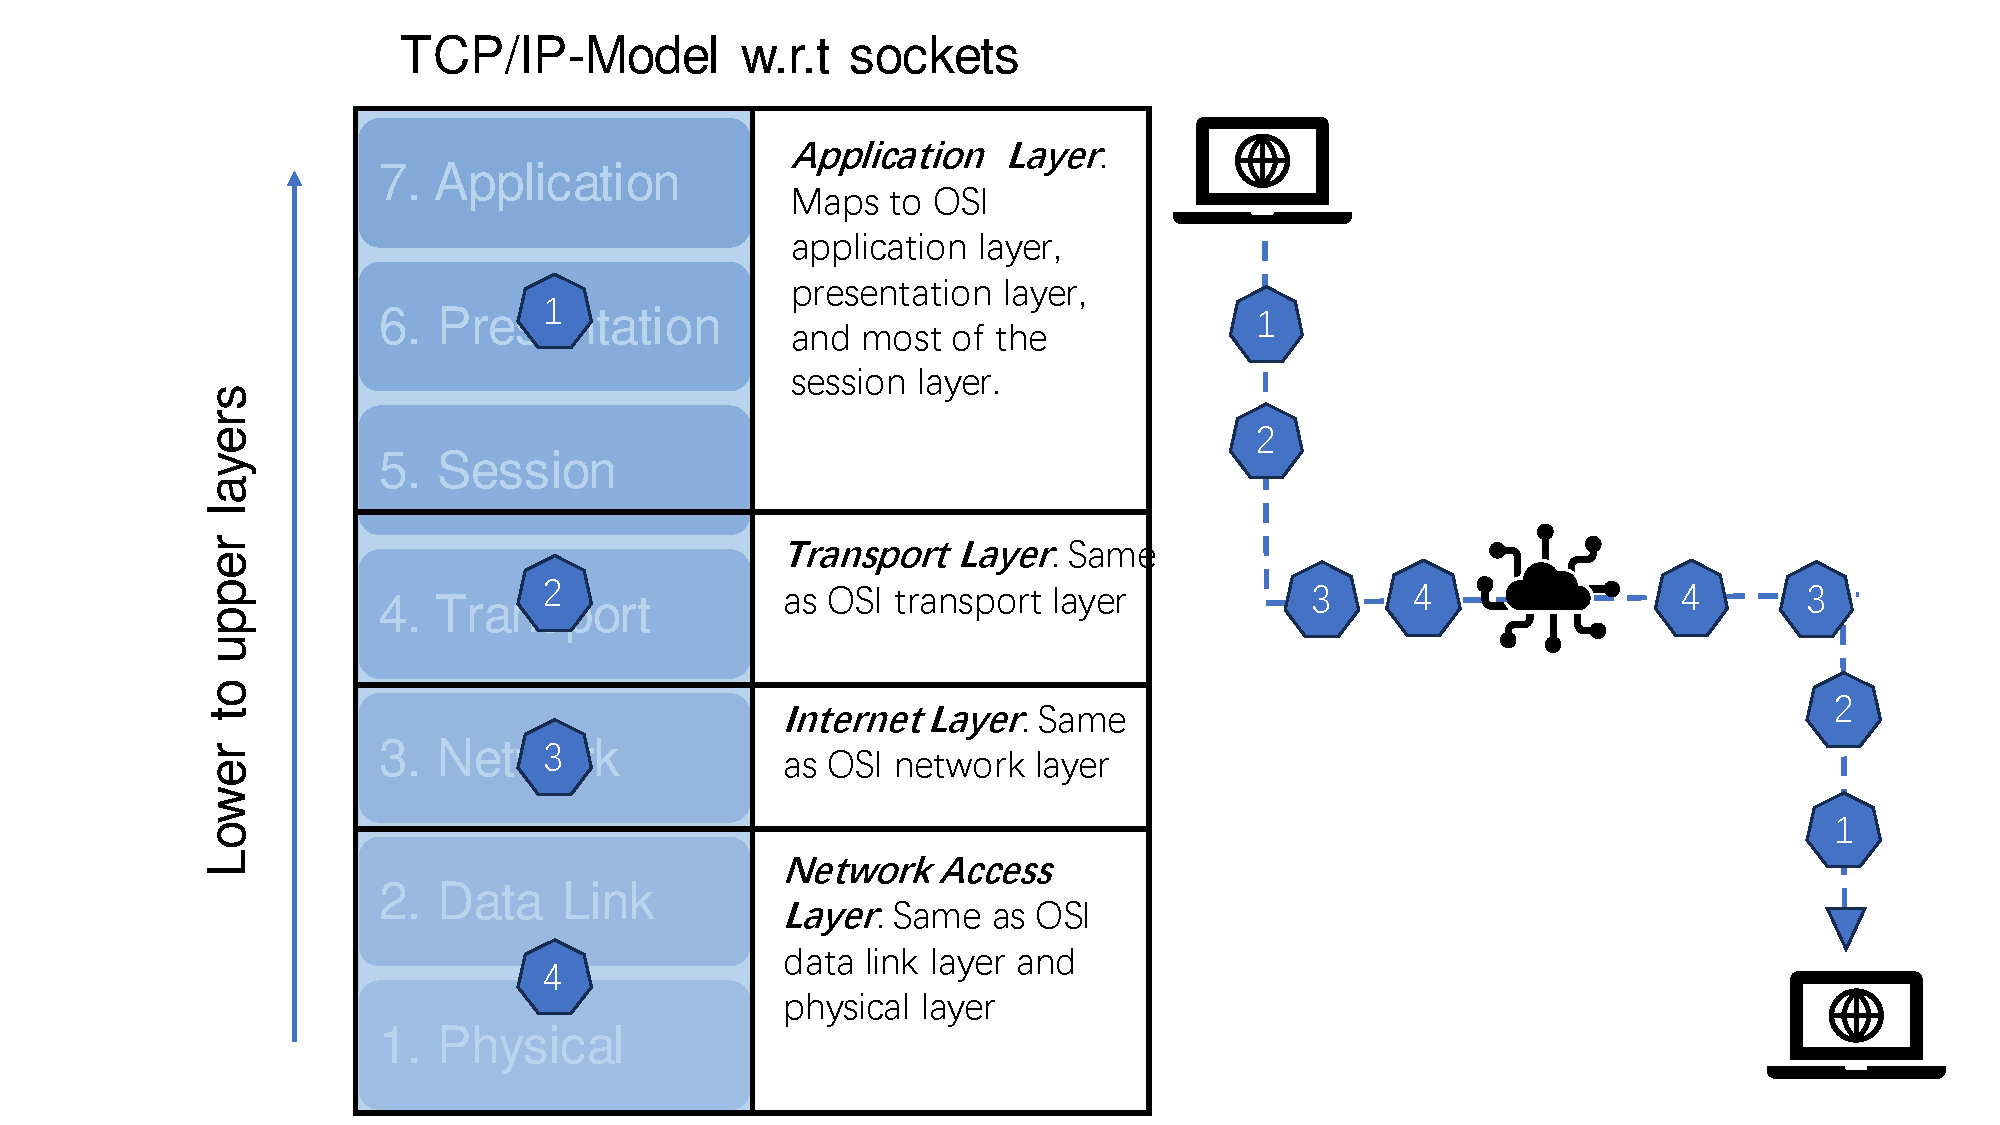
\includegraphics[width=\textwidth]{figures/TCP_IP.pdf}
    \caption{\gls{tcp/ip} model with example protocols. \label{fig: TCP_IP}}
\end{figure}

\subsection{Timing properties of data transport w.r.t sockets and visual notations based on \gls{tcp/ip} model}
When operating in an application, both TCP sockets and WebSockets transport packets 
through all layers of the TCP/IP model. In order to better modularize delay, a set of 
visual notations based on \gls{dsl} is created.
Thanks to the works of former researchers, there are already some commercial graphical tools 
developed for different purposes. The graphical tools 
can be roughly divided into two types: tools ideal for real-world delay measurement, 
for example, the famous Wireshark, OPNET, and NS-3, 
and tools suitable for modeling and visualization, such as OpenModelica, 
Matlab/Simulink and LabVIEW.


Fig.\ref{fig: DSLConceptual} shows a conceptual diagram of a modularized 
general \gls{mas} based on the previous \gls{dsl} design \cite{hujo_toward_2022} 
for industrial \gls{cps} and \gls{dsl} design for robot-like 
systems\cite{volpert_supporting_nodate}. 
Although out of the scope of this thesis, the measurement of delay within 
each layer of \gls{tcp/ip} model will be essential for future investment.
For instance, as depicted in fig.\ref{fig: DSLConceptual}, the delay in 
each layer is represented as a block based on \gls{dsl}, which can be later integrated 
with graphical tools.
In this case, delay in a specific \gls{tcp/ip} layer will become comparable between 
application or transport layer protocols, for example, 
\gls{tcp} and WebSocket. In the graph, \gls{cda} and \gls{dta} 
have the same modular design for the network traffic based on \gls{tcp/ip} 
model. The data transport starts from the \gls{cpu} module on the left-hand side. 
\gls{cpu} is responsible for preparing the data for transmission over the network, 
assigning ports and \gls{ip} addresses, and many more. After a function call 
through a programming language and platform-specific application 
networking API, a socket is created to initialize the network communication. 
During the data transmission, each layer of \gls{tcp/ip} except the lowest 
produces delays 
based on its protocol. Take \gls{cda} as an example; delays in the application, 
transport, and internet layer are based on WebSocket, \gls{tcp}, and 
\gls{ip} protocol. With regard to the delay in the network access layer, it is mainly 
based on the hardware and physical medium. After passing through the network 
environment, the packet is routed in a reverse direction back to other agents, 
for example, a \gls{ra}, to reach the socket endpoint.  



Apart from the network delay of communication between 
agents, as shown in fig.\ref{fig: DSLConceptual}, there is also another 
delay that can be modularized in 
the context of robot control. The robot control systems first introduce a processing 
delay in the robot controller and minor delays of both the network interface and 
\gls{d/a} converter within the I/O module before activating 
the actuator. The network interface refers to the network access layer because of 
the physical interconnections between the robot controller interface and \gls{d/a} converter. 
Afterward, delays in the actuator are produced by a multiplexer and an operating element. 
For each robot state update during the technical process, the data will be recorded 
by the measuring element of the sensor, and the analog signals will be 
converted into a single line with the multiplexer. The signal will then be routed 
back to the robot controller interface through a \gls{a/d} converter and network interface. 








\begin{figure}[htb]
    \centering
    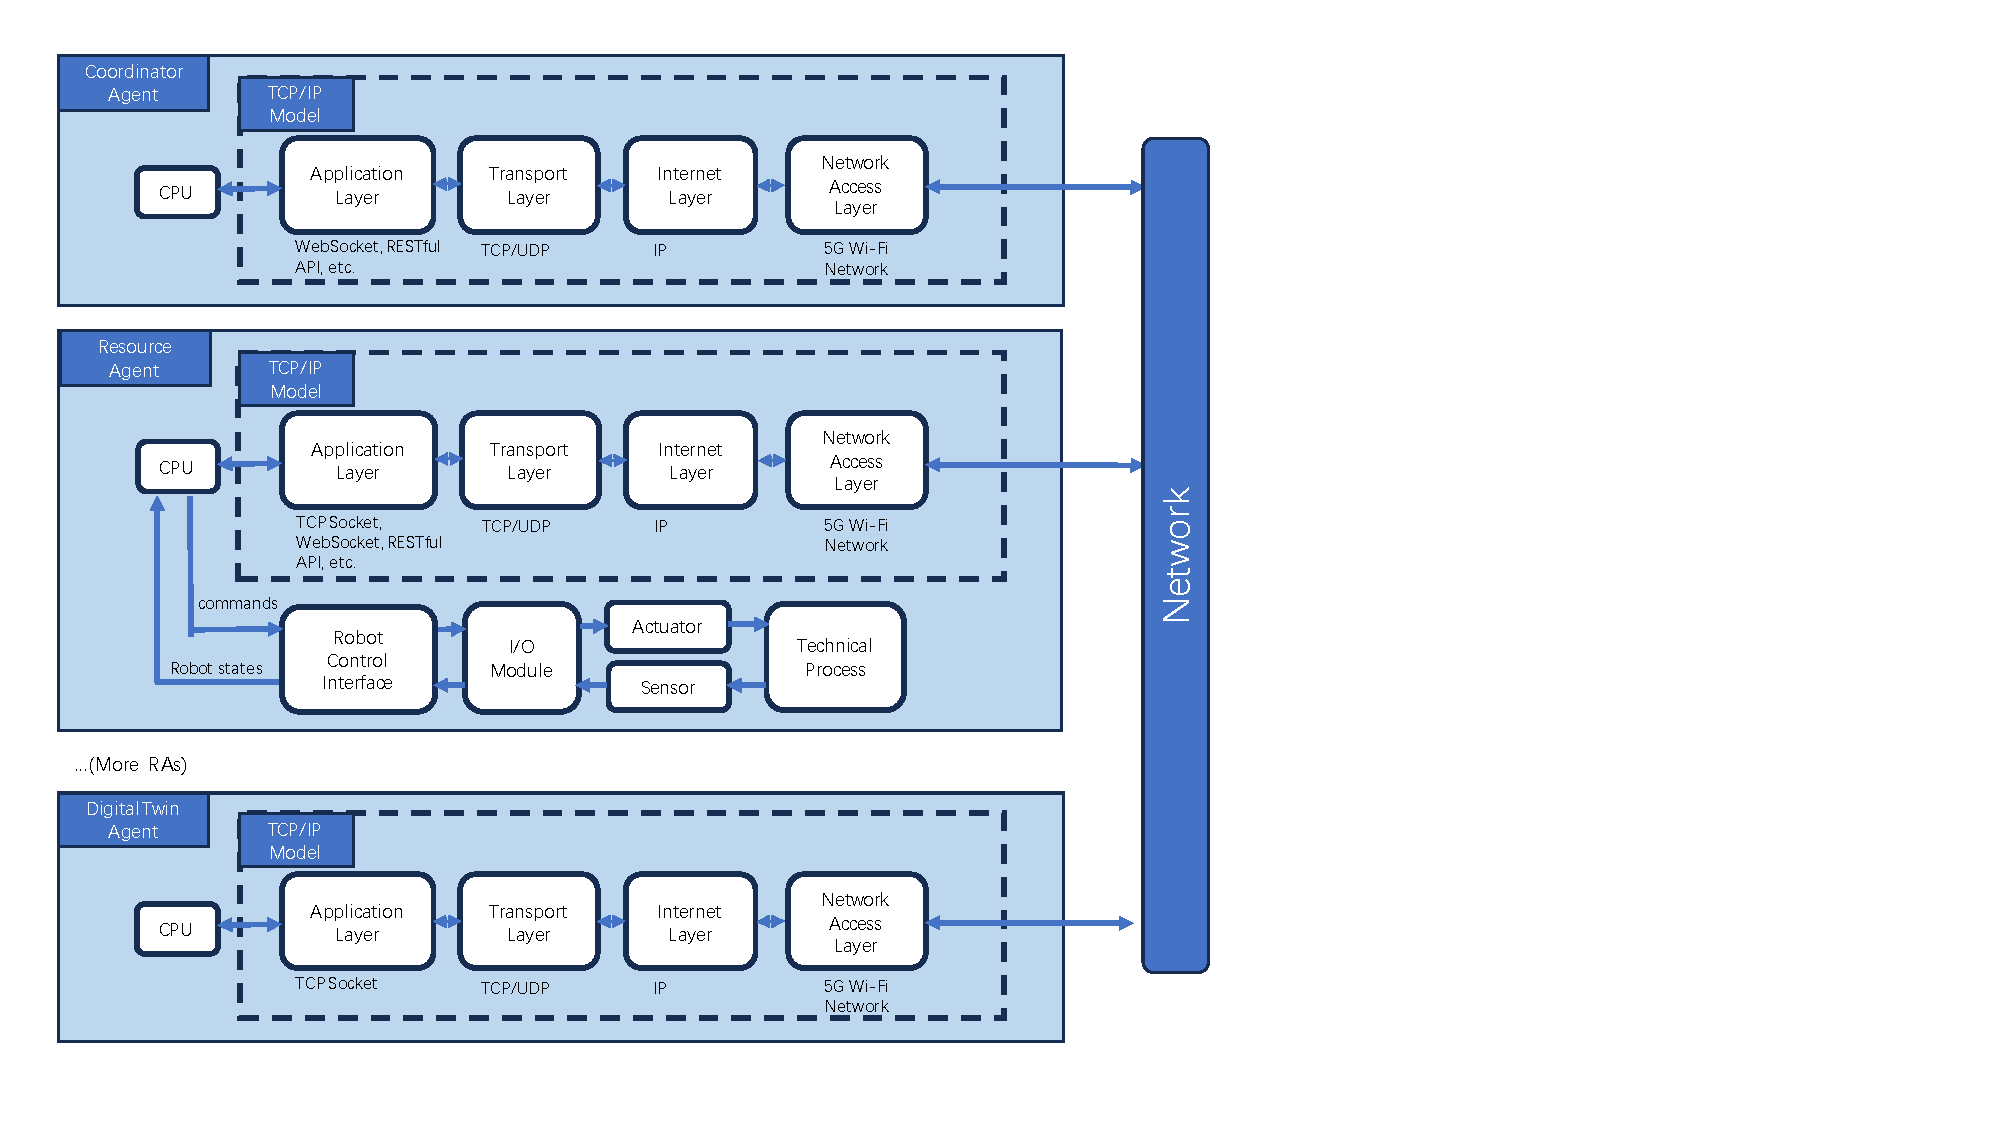
\includegraphics[width=\textwidth]{figures/DSLConceptual.pdf}
    \caption{Conceptual diagram of a modularized general \gls{mas} based on \gls{dsl}. \label{fig: DSLConceptual}}
\end{figure}
        